\documentclass[12pt, a4paper]{report}

% Packages
\usepackage[top=1in, bottom=1in, left=1.5in, right=1in, headheight=15pt]{geometry}
\usepackage{graphicx}
\usepackage{setspace}
\usepackage{times}
\usepackage{fancyhdr}
\usepackage{tocloft}
\usepackage{titlesec}
\usepackage{caption}
\usepackage{booktabs}
\usepackage{array}
\usepackage{longtable}
\usepackage{hyperref}
\usepackage{amsmath}
\usepackage{amssymb}
\usepackage{enumitem}
\usepackage{parskip}
\usepackage[utf8]{inputenc}
\usepackage[T1]{fontenc}
\usepackage{multirow}
\usepackage{pgfgantt}
\usepackage{rotating}
\usepackage{lscape}
\usepackage{xcolor}
\usepackage{tikz}
\usepackage{chngcntr}
\usepackage{float}
\usepackage{tabularx}
\usetikzlibrary{shapes.geometric,arrows.meta,positioning}

% Hyperref setup
\hypersetup{
    colorlinks=true,
    linkcolor=black,
    urlcolor=black,
    citecolor=black,
    plainpages=false,
    hypertexnames=false
}

% Line spacing
\onehalfspacing

% Header and footer
\pagestyle{fancy}
\fancyhf{}
\fancyhead[R]{\thepage}
\renewcommand{\headrulewidth}{0pt}

% Chapter title formatting
\titleformat{\chapter}[block]
  {\normalfont\large\bfseries\raggedright}
  {\thechapter.}{0.5em}{\large\bfseries}

\titlespacing*{\chapter}{0pt}{-20pt}{20pt}

% Section formatting
\titleformat{\section}
  {\normalfont\normalsize\bfseries}
  {\thesection}{1em}{}
\titlespacing*{\section}{0pt}{12pt}{6pt}

% Subsection formatting
\titleformat{\subsection}
  {\normalfont\normalsize\bfseries}
  {\thesubsection}{1em}{}
\titlespacing*{\subsection}{0pt}{10pt}{4pt}

% TOC settings
\setcounter{tocdepth}{3}
\setcounter{secnumdepth}{3}

% Table of contents formatting
\renewcommand{\cftchappresnum}{Chapter }
\renewcommand{\cftchapaftersnum}{.}
\setlength{\cftchapnumwidth}{6em}

% Figure / table / equation numbering reset per chapter, displayed in Roman numerals
\counterwithin{figure}{chapter}
\counterwithin{table}{chapter}
\numberwithin{equation}{chapter}

% TikZ flowchart styles (shared by Figures I, II, III in Chapter 3)
\tikzset{
  fc_startstop/.style={ellipse, draw, thick, fill=blue!8, minimum width=2.1cm, minimum height=0.9cm, align=center, font=\small},
  fc_process/.style={rectangle, draw, thick, fill=orange!8, minimum width=2.6cm, minimum height=1cm, align=center, font=\small},
  fc_decision/.style={diamond, draw, thick, fill=yellow!12, aspect=2.2, align=center, font=\small, inner sep=1pt},
  fc_io/.style={trapezium, trapezium left angle=70, trapezium right angle=110, draw, thick, fill=green!8, align=center, font=\small, minimum width=2.4cm, minimum height=0.9cm},
  fc_sub/.style={rectangle, draw, thick, fill=white, minimum width=3.2cm, minimum height=0.9cm, align=center, font=\small},
}

\begin{document}

% Title Page
\begin{titlepage}
\begin{center}

\begin{figure}[h!]
\centering

\includegraphics[width=3cm]{Images/ncelogo.jpg}
\end{figure}

\vspace{0.3cm}

{\large \textbf{TRIBHUVAN UNIVERSITY}} \\[0.2cm]
{\large \textbf{INSTITUTE OF ENGINEERING}} \\[0.2cm]
{\large \textbf{NATIONAL COLLEGE OF ENGINEERING}} \\

\vspace{1.0cm}

{\large \textbf{A}} \\[0.3cm]

{\large \textbf{MINOR PROJECT MID-TERM REPORT}} \\[0.3cm]


{\large \textbf{ON}} \\[0.3cm]

{\large \textbf{SWASTHYA-EHR}} \\[0.3cm]
{\large \textbf{}} \\

\vspace{2.0cm}

{\normalsize \textbf{SUBMITTED BY:}} \\[0.4cm]
{\normalsize AAYUSH RANJITKAR \hspace{2.0cm} (NCE080BCT003)} \\[0.2cm]
{\normalsize ADITYA BAJRACHARYA \hspace{1.4cm} (NCE080BCT005)} \\[0.2cm] % Updated roll number suffix to 006 (Verify if correct!)
{\normalsize BIRAJ KARKI \hspace{3.3cm} (NCE080BCT011)} \\[0.3cm]
{\normalsize KUSHAL ACHARYA \hspace{2.2cm} (NCE080BCT021)} \\

\vspace{1.0cm}

{\normalsize \textbf{SUBMITTED TO:}} \\[0.4cm]
{\normalsize DEPARTMENT OF ELECTRONICS \& COMPUTER ENGINEERING} \\[0.2cm]
{\normalsize NATIONAL COLLEGE OF ENGINEERING} \\[0.2cm]
{\normalsize LALITPUR, NEPAL} \\

\vspace{1.0cm}

{\normalsize \textbf{JULY, 2026}}

\end{center}
\end{titlepage}





% Front matter: roman numerals
\pagenumbering{roman}
\setcounter{page}{1}

% Acknowledgements
\chapter*{Acknowledgements}
\addcontentsline{toc}{chapter}{Acknowledgements}

We express our sincere gratitude to the Department of Electronics and Computer Engineering at the National College of Engineering for providing the essential academic environment, facilities, and institutional support required to undertake this minor project. The technical ecosystem and learning resources provided by the department were foundational to our progress.

We are deeply indebted to our project supervisor, Mrs.Sharmila Bista, for her constant guidance, critical insights, and patient mentorship at every stage of development. Her constructive feedback was invaluable in navigating technical challenges and refining our project's implementation.

Finally, we extend our heartfelt thanks to our families, friends, and peers for their continuous encouragement and moral support throughout this journey. We appreciate everyone who, directly or indirectly, contributed to the successful execution of this project.
\vspace{2cm}
\noindent

Aayush Ranjitkar \hfill NCE080BCT003 \\
Aditya Bajracharya \hfill NCE080BCT005 \\
Biraj Karki \hfill NCE080BCT011 \\
Kushal Acharya \hfill NCE080BCT021

\newpage

% Table of Contents
\tableofcontents
\newpage

% List of Figures
\listoffigures
\addcontentsline{toc}{chapter}{List of Figures}
\newpage

% List of Tables
\listoftables
\addcontentsline{toc}{chapter}{List of Tables}
\newpage

% List of Abbreviations
\chapter*{List of Abbreviations}
\addcontentsline{toc}{chapter}{List of Abbreviations}

\begin{tabbing}
\hspace{3cm} \= \kill
API \> Application Programming Interface \\
BCT \> Bachelor in Computer Engineering \\
CPU \> Central Processing Unit \\
CRUD \> Create, Read, Update, Delete \\
CSS \> Cascading Style Sheet \\
CSV \> Comma Separated Values \\
HTML \> HyperText Markup Language \\
HTTP \> HyperText Transfer Protocol \\
ID \> Identifier \\
JWT \> JSON Web Token \\
RBAC \> Role-Based Access Control \\
ORM \> Object Relational Mapper \\
OTP \> One Time Password \\
RAM \> Random Access Memory \\
REST \> Representational State Transfer \\
SDLC \> Software Development Life Cycle \\
LOINC \> Logical Observation Identifiers Names and Codes \\
SQL \> Structured Query Language \\
UI \> User Interface \\

\end{tabbing}

\newpage

% Switch to arabic numerals for main content
\pagenumbering{arabic}
\setcounter{page}{1}

%----------------------------------------------------------------------
% CHAPTER 1: INTRODUCTION
%----------------------------------------------------------------------
\chapter{Introduction}

\section{Project Background and Context}

Nepal’s healthcare infrastructure comprises a complex mix of public hospitals, private clinics, and independent diagnostic labs that continue to operate largely in paper-based or heavily fractured environments. Within this traditional framework, critical medical records are not digitally stored, forcing institutions to rely on physical paper files, handwritten prescriptions, and manual ledger logging. Because these local doctors, diagnostic labs, and clinical facilities are entirely unintegrated, there is no structural pipeline to exchange or sync patient information across institutional boundaries. 

Consequently, physicians lack any systematic mechanism for tracking the progression of chronic diseases or assessing a patient’s comprehensive past medical history. When a patient migrates between facilities, clinical record sharing is exceptionally difficult, often requiring the physical transportation of paper folders and film sheets. Furthermore, because data is trapped on paper or within obsolete, isolated databases, there is no structured patient data to export into other external EHR networks or modern health repositories. This systemic lack of coordination forces clinicians to rely completely on patient recall, leading to widespread diagnostic errors, dangerous drug-allergen collisions, and redundant, costly laboratory testing.

The Fast Healthcare Interoperability Resources (HL7 FHIR) standard resolves this foundational bottleneck by providing a universal, modular data model for core clinical resources. Built on a lightweight RESTful architecture utilizing open JSON payloads, FHIR serves as the modern global benchmark for converting disconnected workflows into interoperable health information exchanges. 

The SwasthyaEHR project directly targets these systemic vulnerabilities by implementing this global standard within a multi-institution network model. Built upon a decoupled React frontend and a Django REST Framework backend backed by PostgreSQL, the system bridges existing infrastructural gaps. It introduces a functional blueprint for secure interoperability, featuring centralized Role-Based Access Control (RBAC) middleware to securely partition duties among doctors, lab technicians, and pharmacists, alongside an atomic clinical safety interceptor that actively evaluates patient allergy profiles to halt conflicting medical transactions in real time.


\clearpage
\section{Problem Statement}
The development of SwasthyaEHR is motivated by the following core challenges within Nepal's contemporary health informatics landscape:
\begin{itemize}
    \item Medical institutions independently store patient records using disparate database schemas and contrasting data structures.
    \item The absence of global data standardization frameworks—specifically the HL7 FHIR protocol—makes secure, cross-institutional data exchange virtually impossible.
    \item Fragmented histories force clinicians to rely on duplicate diagnostic tests due to inaccessible past records.
    \item Disconnected backend databases lack a unified validation engine capable of executing automated, cross-institutional safety checks.
    \item Without real-time transaction interceptors, systems cannot reliably perform live sweeps to flag drug-allergen collisions or trigger critical allergy warnings.
    \item Current clinical workflows lack a clean separation of duties between doctors, lab technicians, pharmacists, and receptionists, leading to auditing gaps.
    \item Patients are frequently restricted from transparent access to their own medical histories, preventing active self-registration and profile management.
    \item The ecosystem lacks a unified way to aggregate, serialize, and track multi-institutional clinical observations over time.
\end{itemize}

\clearpage
\section{Objectives}


\subsection{Specific Objectives}
To develop a standardized, secure, and interoperable Electronic Health Record (EHR) web application utilizing the HL7 FHIR framework to achieve seamless longitudinal clinical data exchange and safety-focused patient care across multiple simulated health institutions in Nepal.

\subsection{General Objective}
\begin{enumerate}[label=\Roman*.]
    \item To model and implement a decoupled, three-tier architecture utilizing a React SPA frontend and a Django with Django REST Framework (DRF) backend database engine.
    \item To design an interoperability layer capable of serializing relational PostgreSQL records into standardized, read-only HL7 FHIR R4 clinical resources (Patient, Observation, and Bundle).
    \item To develop a transactional Clinical Safety Interceptor engine that performs atomic, case-insensitive substring matching against JSONB allergy arrays to prevent conflicting medical prescriptions.
    \item To implement a strict Role-Based Access Control (RBAC) authorization matrix securing administrative, medical professional, and patient-scoped endpoint views.
    
   
\end{enumerate}
\clearpage
\section{Scope}
The scope of this minor project includes:

\begin{enumerate}[label=\Roman*.]
  \item Engineering core functional workflows for managing patient registrations, physician lab orders, numerical lab observations, and medication prescriptions.
  \item Patient and lab data can be exported as standards-compliant *FHIR R4* JSON resources, allowing the data to be understood by any other FHIR-compatible health system — the key "interoperability" objective of the project.
  \item Implementing a server-side transactional safeguard that automatically scans a patient's historical allergen records to block conflicting or unsafe prescriptions before they are saved.
  \item Setting up a strict authorization structure using JWT tokens to securely separate accessible endpoints and dashboards based on distinct user roles, including Administrators, Doctors, Lab Technicians, Pharmacists, and Patients.
  \item Designing a frontend data charting interface using Chart.js to aggregate and graph a patient's laboratory values over time, even when collected from different simulated institutions.
  \item Patients can be registered two ways — self-registration from a public web form, or by a receptionist at the front desk. Every patient receives a UUID internal key and a human-readable hospital ID (HOSP-YYYY-NNNNN).
\end{enumerate}


%----------------------------------------------------------------------
% CHAPTER 2: LITERATURE REVIEW
%----------------------------------------------------------------------
\chapter{Literature Review}

\section{Related Work}

Bates et al. \cite{bates1,bates2} investigated the impact of information technology and computerized physician order entry systems on improving patient safety and reducing medication-related errors in healthcare environments. Their studies demonstrated that electronic health records not only improve documentation quality but also significantly reduce preventable clinical errors through automated clinical workflows and decision support mechanisms. Adler-Milstein et al. \cite{adler} further reported that although electronic health record adoption has increased considerably, advanced and meaningful utilization remains inconsistent across healthcare institutions. These findings highlight that the true value of electronic health records lies beyond digitization, requiring integrated clinical safety mechanisms. This work directly motivated the development of SwasthyaEHR as a patient-centered electronic health record system that combines digital record management with automated prescription safety validation.

Bender and Sartipi \cite{bender} introduced HL7 Fast Healthcare Interoperability Resources (FHIR) as a lightweight, RESTful standard for exchanging healthcare information between heterogeneous information systems. Mandel et al. \cite{mandel} further demonstrated through the SMART on FHIR framework that standardized web APIs combined with secure authentication protocols enable interoperable healthcare applications while preserving patient privacy and fine-grained access control. The HL7 FHIR R4 specification \cite{hl7spec} standardized healthcare resources such as Patient, Observation, MedicationRequest, and Bundle using JSON-based representations for efficient data exchange. These studies directly influenced the SwasthyaEHR system architecture by adopting FHIR R4 resources, RESTful APIs, and standardized clinical data serialization to achieve interoperability across healthcare systems.

Kuperman et al. \cite{kuperman} reviewed medication-related clinical decision support systems and demonstrated that computerized prescription validation significantly improves medication safety by detecting adverse drug events before clinical administration. However, van der Sijs et al. \cite{vandersijs} observed that clinicians frequently override computerized drug safety alerts, while Topaz et al. \cite{topaz} reported increasing drug-allergy alert override rates in electronic health record systems over time. These studies emphasized the importance of designing high-specificity clinical safety mechanisms that minimize unnecessary alerts while preventing potentially harmful prescriptions. Their findings directly influenced the Clinical Safety Interceptor implemented in SwasthyaEHR, where prescriptions are automatically validated against documented patient allergies and unsafe medications are blocked before database transactions are completed.

\cite{possible} Demonstrated the successful deployment of OpenMRS and Bahmni-based electronic health record systems within rural healthcare facilities in Nepal, improving patient record management and continuity of care. At the national level, Nepal's Health Management Information System based on DHIS2 \cite{dhis2} and the Ministry of Health and Population \cite{mohp}, together with the World Health Organization's Global Strategy on Digital Health \cite{who}, emphasize strengthening digital health infrastructure and standardized healthcare information management. These studies reveal that although Nepal has made considerable progress in digital health reporting, interoperable patient-level electronic health record systems with integrated clinical safety remain limited. This gap directly motivated the development of SwasthyaEHR as a lightweight, role-based, FHIR-enabled electronic health record system incorporating standardized laboratory data exchange and automated prescription safety for healthcare institutions in Nepal.
```

\section{Related Theory}

\subsection{HL7 FHIR Interoperability Standard}
HL7 FHIR (Fast Healthcare Interoperability Resources) is an international data standard engineered by Health Level Seven International to facilitate seamless semantic exchange across heterogeneous medical information ecosystems. Traditional healthcare infrastructure is plagued by highly siloed relational database schemas, preventing reliable cross-institutional data consistency. 

FHIR mitigates this structural friction by encapsulating discrete healthcare concepts into modular units known as "Resources." In the SwasthyaEHR platform, cross-institutional data integration leverages three foundational FHIR resource boundaries:
\begin{itemize}
    \item \textbf{Patient Resource:} Encapsulates core demographic tracking attributes and verified identification markers.
    \item \textbf{Observation Resource:} Serves as the programmatic container for clinical laboratory measurements, vital signs, and numeric assessments.
    \item \textbf{Bundle Resource:} Operates as a container document payload to aggregate multiple distinct resource instances into a single transactional exchange.
\end{itemize}

These structured objects are queried and transmitted utilizing a stateless RESTful architecture over standard Hypertext Transfer Protocol (HTTP) vectors. The default routing hierarchy for parsing a specific clinical profile follows the standardized endpoint template:
\begin{equation}
    \texttt{GET\ /[resourceType]/[id]}
\end{equation}

During cross-institutional ingestion, incoming relational rows are mapped dynamically into valid FHIR JSON representations. The application layer handles this translation by mapping fields from a relational laboratory data object $L$ into a compliant FHIR Observation payload $O$ through the following systemic definitions:
\begin{equation}
    O\text{.code} = \text{LOINC}(L\text{.test\_name})
\end{equation}
\begin{equation}
    O\text{.valueQuantity} = \{ \text{value}: L\text{.result\_value},\ \text{unit}: L\text{.unit\_marker} \}
\end{equation}
\begin{equation}
    O\text{.subject} = \text{Reference}(\texttt{Patient/} + L\text{.patient\_uuid})
\end{equation}

\subsection{Role-Based Access Control (RBAC)}
Role-Based Access Control (RBAC) represents a strict authorization architecture where system operation permissions are linked directly to explicit institutional roles rather than being decoupled at the individual user profile level. To protect sensitive health records within SwasthyaEHR, five operational system boundaries are enforced:
\begin{itemize}
    \item \textbf{Administrator:} Grants total administrative data control, system health logging, and auditable track access.
    \item \textbf{Doctor:} Authorizes the verification of medical histories, creation of lab orders, and writing of medication prescriptions.
    \item \textbf{Lab Technician:} Restricts interface capabilities to the uploading and formatting of raw numerical laboratory results.
    \item \textbf{Pharmacist:} Allows read-only access to active prescriptions and verification logs to complete medicine dispensing.
    \item \textbf{Patient:} Provides direct read-only access to personal longitudinal charts, laboratory results, and historical logs.
\end{itemize}

Stateless endpoint authentication is established utilizing cryptographically signed JSON Web Tokens (JWT). Upon verification of user credentials, the application server issues an encoded token incorporating the user’s role and access scope. Subsequent client-side API requests must provide this bearer token within the HTTP authorization header. Access authorization is calculated via a logical evaluation function before data is returned:
\begin{equation}
    \text{Access} = f(\text{UserRole},\ \text{EndpointScope},\ \text{TokenValidity})
\end{equation}

\subsection{Transactional Clinical Safety Logic}
The prescription validation engine implements automated safeguards to intercept and block preventable adverse drug events before records are written to persistent storage. This is managed by evaluating incoming prescriptions against a patient's known allergy history using strict substring evaluation logic inside an isolated, server-side transactional boundary. 

Let $P_{\text{drug}}$ represent the incoming prescription molecule identifier text string, and let $A = \{a_1, a_2, \dots, a_n\}$ represent the text array of a patient's historical recorded allergens extracted from a PostgreSQL JSONB data column. The safety coefficient $S$ for any given prescription transaction is defined as follows:
\begin{equation}
    S = \prod_{i=1}^{n} \sigma(P_{\text{drug}},\ a_i)
\end{equation}
where the binary mismatch indicator function $\sigma(P_{\text{drug}},\ a_i)$ evaluates string intersections independently of text casing variations:
\begin{equation}
    \sigma(P_{\text{drug}},\ a_i) = 
    \begin{cases} 
        0 & \text{if\ } a_i \text{\ is\ a\ substring\ of\ } P_{\text{drug}} \\ 
        1 & \text{otherwise} 
    \end{cases}
\end{equation}

A database transactional write command is only permitted to proceed if the complete sequence resolves to a safe state ($S = 1$). If the interceptor detects a conflict ($S = 0$), a severe clinical collision state is identified, and the transaction is aborted via an immediate atomic rollback operation. The system parameter boundaries governing these system rules are defined in Table 2.1.

\begin{table}[h!]
\centering
\caption{Clinical Safety and System Execution Parameters}
\label{tab:safety_parameters}

\resizebox{\textwidth}{!}{%
\begin{tabular}{llll}
\hline
\textbf{System Component} & \textbf{Core Variables} & \textbf{Data Strategy} & \textbf{Execution Target} \\ \hline
FHIR Serialization & Patient, Observation, Bundle & Relational to JSON & On-the-fly Representation \\
Access Protection & JWT Signature, Role Scopes & Bearer Token Filter & Middleware Layer Intercept \\
Safety Interceptor & Drug String, Allergen Array & Substring Matching & Atomic DB Transaction \\
\hline
\end{tabular}
}
\end{table}



\subsection{Standardized Clinical Terminologies}
Uniform terminology systems ensure that data exchanged between independent clinical sites can be universally understood, preventing semantic fragmentation caused by divergent naming styles on local data capture forms.

\textbf{LOINC (Logical Observation Identifiers Names and Codes):} LOINC represents the international standard for classifying laboratory tests and clinical observation definitions. It provides unique codes that precisely identity the medical question asked. In SwasthyaEHR, all laboratory results submitted by technicians are mapped to an official LOINC code, allowing the backend to unify disparate localized lab aliases (such as \textit{"Blood Sugar"}, \textit{"Fasting Glucose"}, or \textit{"RBS"}) under a single, trackable timeline.

\textbf{SNOMED CT (Systematized Nomenclature of Medicine Clinical Terms):} SNOMED CT is a comprehensive clinical terminology system designed to index diagnoses, clinical findings, and anatomical details. While LOINC registers the exact clinical observation test, SNOMED CT codes classify the clinical state or diagnosis resulting from that test. This structure provides a predictable vocabulary that allows clinical outcomes to be successfully evaluated by external semantic frameworks.

\subsection{Representational State Transfer (REST) Architecture}
Representational State Transfer (REST) is an architectural style designed for distributed hypermedia systems. In a RESTful architecture, any clinical entity within the health system—such as a patient identity, an electronic prescription, or a laboratory profile—is treated as a uniquely addressable, network-accessible resource. By enforcing structural constraints like server statelessness, a uniform JSON payload interface, and a clean separation of client-server concerns, REST enables the underlying engineering layer to maximize horizontal scalability. This stateless architecture dictates that every incoming request carries its own cryptographic context, eliminating server-side session reliance and ensuring that disparate medical facilities can communicate reliably without maintaining continuous, memory-intensive backend connections.

\subsection{The Django Web Framework}
The backend engineering layer utilizes the Django web framework to provide an enterprise-grade development foundation following the Model-View-Template (MVT) layout. Django leans heavily on its advanced Object-Relational Mapping (ORM) layer, which abstracts low-level SQL mechanics into typed, secure data models. This architectural layer inherently eliminates severe systemic vulnerabilities like SQL injection while managing complex schemas across relational instances like PostgreSQL. Within this infrastructure, the ORM handles transactional integrity and automates schema migrations, allowing the database to utilize complex data types, such as PostgreSQL \texttt{JSONB} fields for schema-less data like clinical allergy lists, while maintaining rigid relational linkages for identity verification.

\subsection{Django REST Framework (DRF)}
The Django REST Framework (DRF) functions as an essential middleware layer that translates internal relational database models into secure web services. It executes bi-directional data conversions through serialization pipelines that strictly validate client inputs against internal constraints before database storage. Furthermore, DRF decouples operational control through modular ViewSets and pluggable authentication filters. This allows the application to parse incoming token scopes and enforce granular, server-side Role-Based Access Control (RBAC) that blocks unauthorized data modifications and securely partitions operational access boundaries across varying clinical workflows.

\subsection{The React JavaScript Library}
The client-facing ecosystem is driven by the React JavaScript library, which acts as a declarative, single-page application (SPA) framework designed to ingest and render asynchronous back-end telemetry. React structures user interfaces into self-contained, state-managing components, enabling complex multi-role medical views to decouple their visual logic from direct browser Document Object Model (DOM) mutations. By utilizing an optimized virtual DOM diffing engine, React minimizes re-rendering penalties during intensive clinical data entry workflows, ensuring highly responsive client execution. Data architecture inside the application follows a predictable, unidirectional stream that flows downward via immutable attributes and bubbles modifications upward through callbacks. This separation allows the interface to react instantaneously to changing state parameters—such as live validation blocks or visual real-time allergy alerts.

\subsection{Fast Healthcare Interoperability Resources (HL7 FHIR)}
Bridging the gap between isolated application structures and global medical data portability is the Fast Healthcare Interoperability Resources (FHIR) standard developed by HL7. FHIR represents a modern paradigm shift by translating complex clinical observations into modular, developer-friendly JSON entities known as resources. Guided by the pragmatic 80/20 design rule, the standard optimizes network exchanges by embedding only the most universally common clinical markers directly within base resource structures, offloading specialized workflows onto an extensible profiling framework. Syntactic coordination across disparate healthcare nodes is achieved by binding these open JSON objects to RESTful API endpoints, while semantic consistency is strictly enforced by mapping internal data attributes to universal terminology specifications like LOINC codes for laboratory telemetry. When complex medical histories require cross-institutional collation, FHIR aggregates these distinct granular documents into unified transactional containers known as Bundles. This composite serialization standardizes data exchange pipelines, creating a uniform, standards-compliant middleware matrix capable of driving interoperability throughout the healthcare infrastructure.

%----------------------------------------------------------------------
% CHAPTER 3: METHODOLOGY
%----------------------------------------------------------------------
\chapter{Methodology}

\section{Software Development Model}

The project is developed using the Iterative Model with parallel development across
team members. This model was chosen because the work is split into frontend, backend,and clinical serialization parts that are built at the same time, with each part going throughrepeated cycles of design, build, and test until the full system is ready.
\begin{figure}[H]
\centering
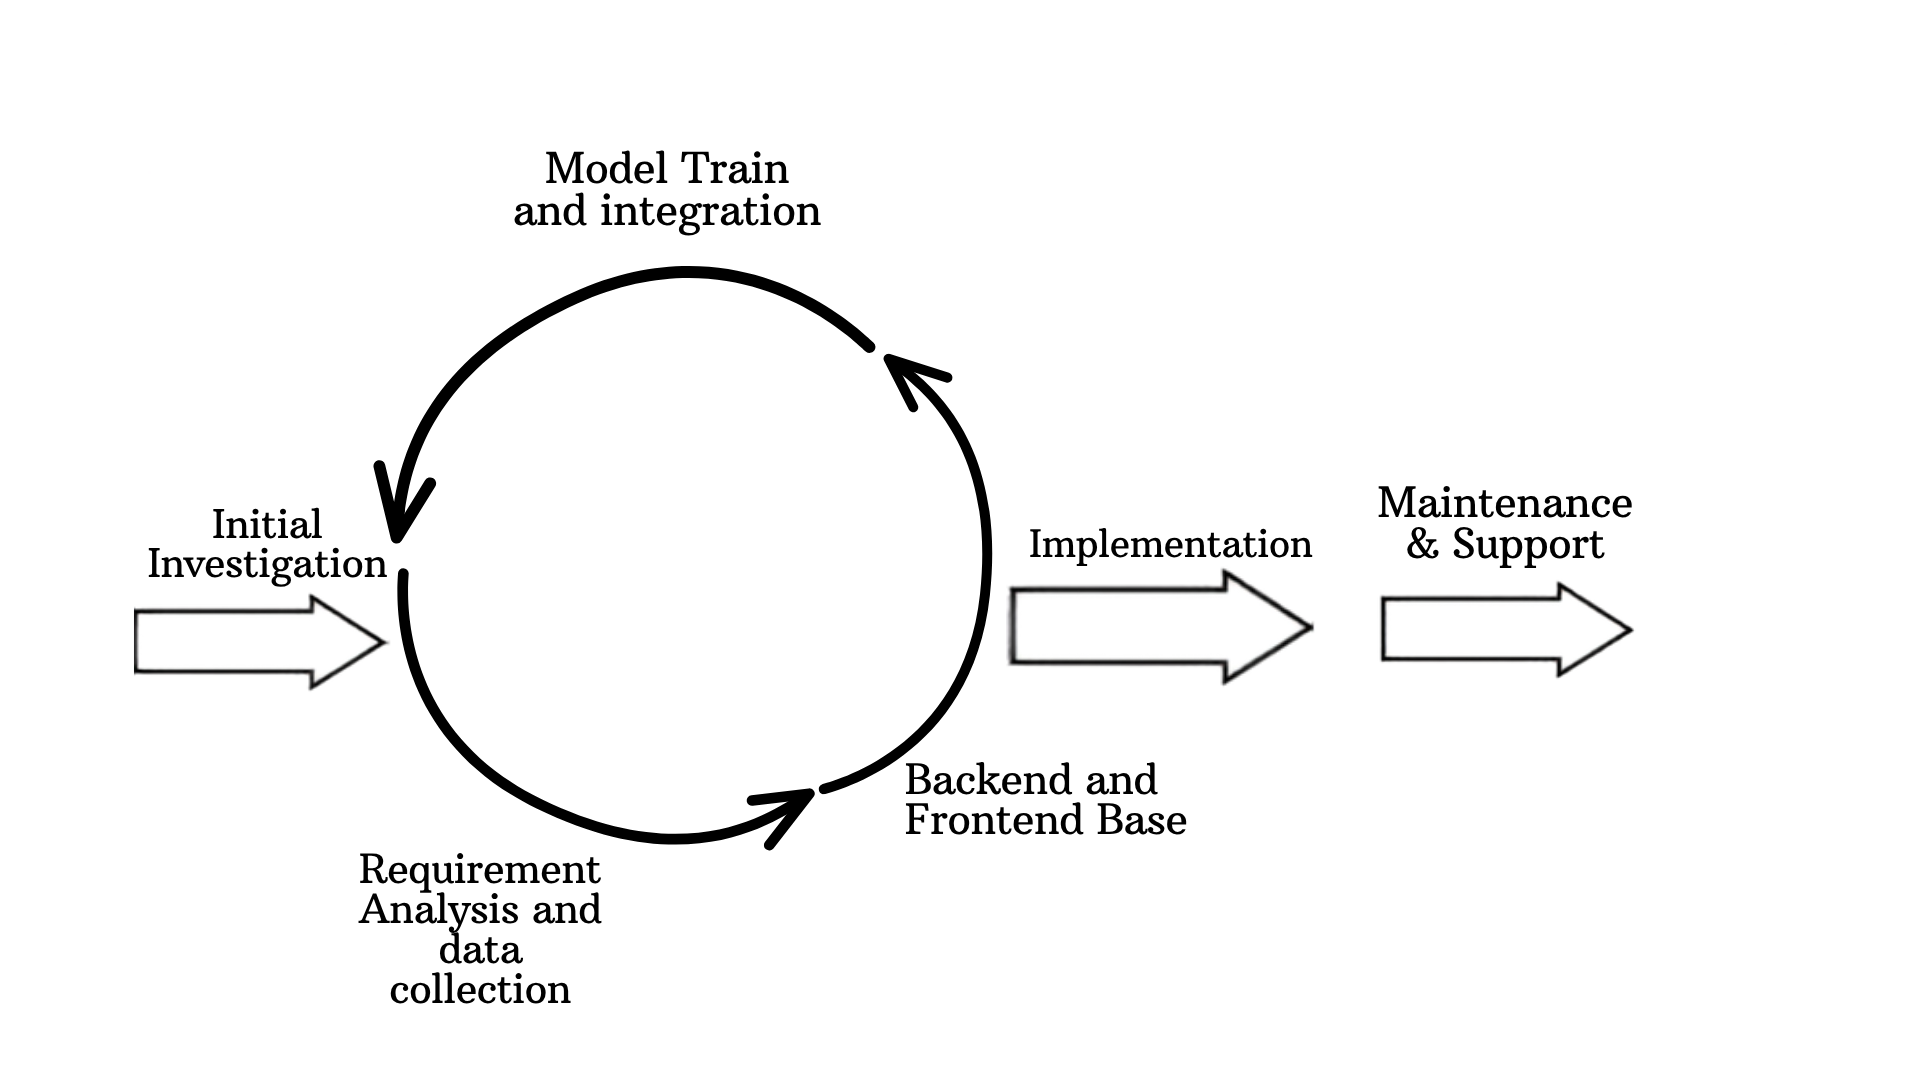
\includegraphics[width=0.9\textwidth]{Images/ITERATIVE_MODEL.png}
\caption{Iterative Software Development Model used in this project}
\label{fig:iterative}
\end{figure}


The Iterative Model is suitable for this project because it allows the system to be devel-
oped in small stages with continuous improvements. The project consists of frontend,
backend, database, and interoperability components, which can be developed and
tested independently while gradually integrating them into a complete system. This
approach allows the team to identify and fix issues early, add new features in each it-
eration, and improve the system based on testing results and feedback from the project
supervisor. It also provides flexibility to refine both the web application and the data mapping
layer throughout the development process.

The project is divided into four short cycles. Each cycle adds a new layer of the system
on top of what already works.
\begin{enumerate}[label=\Roman*.]
    \item \textbf{Iteration 1: Requirement Analysis and Data Collection.} The team gathered
    the project requirements, evaluated the HL7 FHIR R4 standard structures, and mapped out 
    the logical PostgreSQL schema relationships. This was completed before development began.
    \item \textbf{Iteration 2: Backend and Frontend Base.} The Django backend with Django REST 
    Framework (DRF) and the React frontend were built in parallel. The authentication flow, 
    database setup, and basic pages were finished.
    \item \textbf{Iteration 3: Interoperability Mapping and Security Engine.} The custom serialization 
    layer will be implemented to translate relational database records into standardized HL7 FHIR 
    JSON payloads, and the backend Role-Based Access Control (RBAC) matrix will be fully deployed.
    \item \textbf{Iteration 4: Transactional Safety Validation and Testing.} The automated Clinical 
    Safety Interceptor endpoints, the cross-institutional trend visualization charts, and the final 
    system testing will be completed in this cycle.
\end{enumerate}

\section{Requirement Analysis}

\subsection{Functional Requirements}
The functional requirements describe what the system must do. They are grouped by user role.

\noindent \textbf{Patient Functions:}
\begin{itemize}
    \item A new patient must be able to register by providing a full name, an email address, a password, and a password confirmation.
    \item A new patient must receive a six digit code on their email after registration and must enter this code to confirm the account.
    \item A registered patient must be able to log in using email and password.
    \item A patient must be able to reset their password by requesting a verification code on their registered email.
    \item A patient must be able to view their verified longitudinal clinical charts, lab results, and medication history summaries.
    \item A patient must be able to monitor historical trends of key vital measurements aggregated from simulated clinics over time.
    \item A patient must be able to view details of active data access permission grants issued to healthcare providers.
\end{itemize}

\noindent \textbf{Medical Staff Functions (Doctor, Technician, Pharmacist):}
\begin{itemize}
    \item A clinician must be able to log in to a separate workspace dashboard using email and password.
    \item A medical professional must be able to query an active patient record index and view aggregated, cross-institutional health profiles.
    \item A doctor must be able to issue new medical prescriptions and select laboratory tests within the patient routing interface.
    \item A technician must be able to input numerical laboratory results and map them to standard system markers via data entry forms.
    \item A pharmacist must be able to access verified prescription payloads to safely dispense medications and record active completion logs.
\end{itemize}

\noindent \textbf{Admin Functions:}
\begin{itemize}
    \item An admin must be able to view the list of all users registered within the system database.
    \item An admin must be able to add a new user node, update user details, or remove an active account when necessary.
    \item An admin must be able to assign or change the role mapping of any user, such as patient, doctor, technician, pharmacist, or admin.
    \item Only admins must be able to access the central user management and system access configuration pages.
\end{itemize}

\noindent \textbf{System Functions:}
\begin{itemize}
    \item The system must classify request authorization scopes by user role, resource identity, and token verification constraints.
    \item The system must dynamically map flat relational rows into valid HL7 FHIR payloads using backend serialization middleware.
    \item The system must intercept prescription entries inside an atomic transaction block and run substring checks against patient recorded allergens.
    \item The system must store application user parameters, historical FHIR observations, and transactional access logs in the relational database.
\end{itemize}

\subsection{Non Functional Requirements}
The non functional requirements describe how the system performs rather than what it does.
\begin{itemize}
    \item \textbf{Performance.} The system should return FHIR serialization and validation results in under two seconds. Pages should load fast and respond quickly to user actions.
    \item \textbf{Usability.} The interface should be simple and clear. Users should be able to find what they need with only a few clicks, and the layout should work well on both desktop and mobile screens.
    \item \textbf{Reliability.} The system should remain available throughout the day. It should handle temporary backend failures without crashing and should show proper error messages when something goes wrong.
    \item \textbf{Security.} Passwords must be stored in hashed form. One time codes must expire after a fixed time. User sessions must be managed safely, and protected routes must reject users who are not logged in.
    \item \textbf{Scalability.} The system should support future growth in users, observations, and transactions. New FHIR resource definitions should be added without major changes to the existing code.
    \item \textbf{Compatibility.} The website should work on all major browsers and on different screen sizes, including smaller mobile screens.
    \item \textbf{Maintainability.} The codebase should be split into clear modules with proper documentation, coding standards, and version control. Serialization utilities should be managed independently of the frontend display components.
    \item \textbf{Availability.} The system should keep working on slow internet connections without losing the user session or breaking the page layout.
\end{itemize}
\section{Proposed System Design}

\subsection{System Architecture}

\begin{figure}[H]
\centering
\makebox[\textwidth][c]{%
  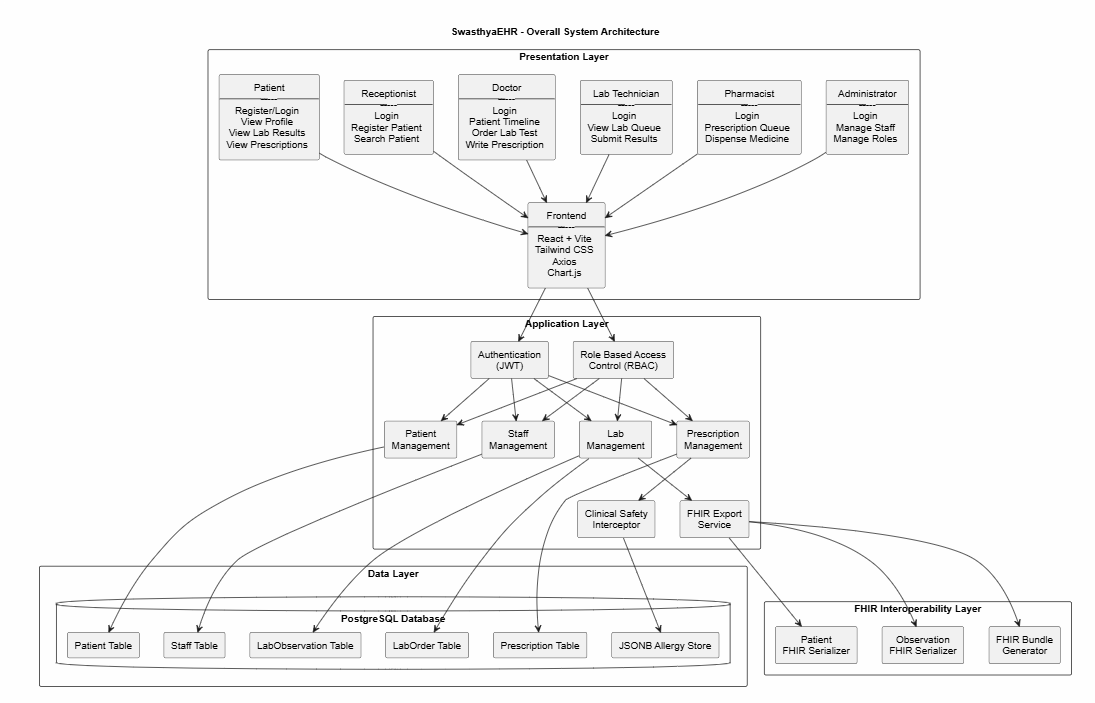
\includegraphics[width=1.25\textwidth,height=12cm,keepaspectratio=false]{Images/systemarchitecture.png}%
}
\caption{System Architecture of the SwasthyaEHR Platform}
\label{fig:systemarchitecture}
\end{figure}
\clearpage

The theoretical design of the SwasthyaEHR platform is founded on a decoupled three-tier software architecture that leverages a state-driven Single Page Application (SPA) frontend to asynchronously stream lightweight JSON data from a Django REST Framework backend, isolating user interactions from heavy server-side processing. Persistent storage is managed by a hybrid PostgreSQL relational cluster that combines standard transactional tables with flexible, indexed JSONB columns to securely log varying clinical metrics like patient allergy histories without schema rigidity. To ensure semantic interoperability across disparate simulated health nodes, the application layer runs an automated ingestion pipeline that maps flat relational database inputs into globally standardized HL7 FHIR R4 resources (such as Patient and Observation blocks) by dynamically translating localized text terms into universal LOINC and SNOMED CT codes. Data privacy and security boundaries are enforced at the network perimeter via stateless JSON Web Token (JWT) authentication evaluated through a middleware-driven Role-Based Access Control (RBAC) matrix that restricts endpoint exposure to explicit institutional roles. Finally, clinical data integrity is protected by an automated, server-side interception engine operating inside strict ACID-compliant database transactions (\texttt{@transaction.atomic}), which uses case-insensitive substring matching to check incoming prescriptions against a patient's historical allergy array, triggering an immediate atomic database rollback to completely wipe out uncommitted writes if a medical conflict is detected.
\subsection{Use Case Diagram}

\begin{figure}[H]
\centering
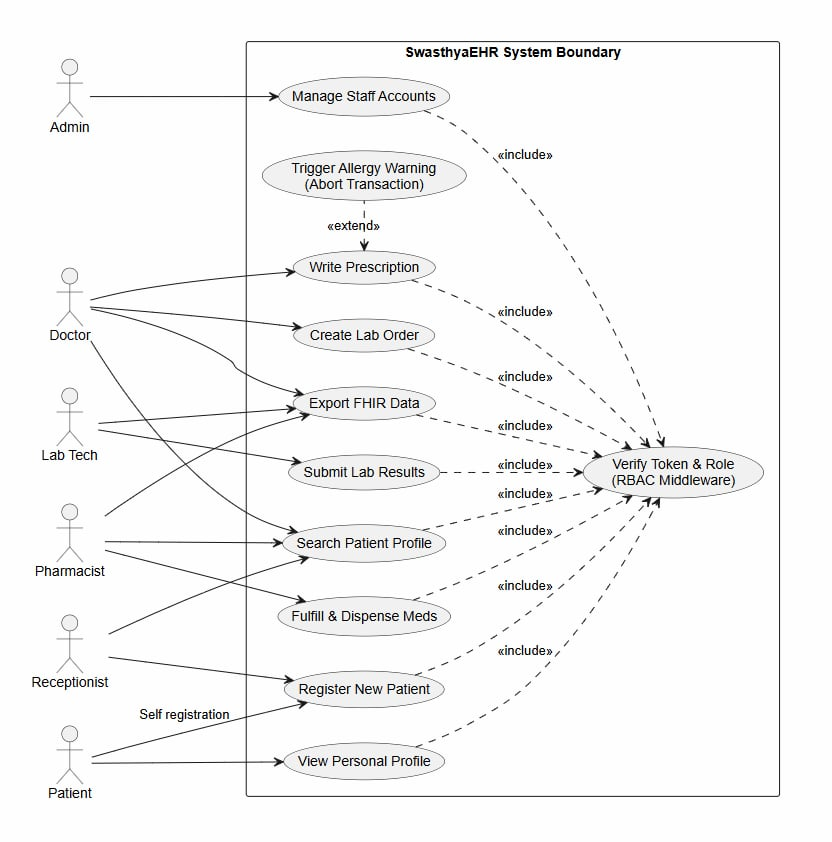
\includegraphics[width=1.0\textwidth]{Images/usecase.png}
\caption{Use Case Diagram of the System}
\label{fig:usecase}
\end{figure}

The use case diagram in Figure \ref{fig:usecase} illustrates how the seven distinct user groups—Admin, Doctor, Lab Tech, Pharmacist, Receptionist, Patient, and the underlying system layer—interact within the defined SwasthyaEHR system boundary. Each actor is mapped directly to their authorized clinical or administrative workflows, establishing a clear separation of duties across the platform. Crucially, rather than duplicating authorization logic across separate endpoints, the system utilizes a centralized base use case, **Verify Token \& Role (RBAC Middleware)**, which is dynamically executed via an included relationship by every secure transaction to enforce token verification at the network perimeter.

Under this security framework, administrative users are restricted to managing staff accounts, while front-desk staff or receptionists are dedicated to registering new patients. Patients themselves can initiate self-registration or authenticate to view their personal profiles. Within the clinical core, doctors retain the widest operational scope, enabling them to create laboratory orders, search patient profiles, export standardized data, and write prescriptions. The writing of a prescription features a critical safety extension, allowing the backend validation engine to automatically trigger an allergy warning and abort the database transaction if a drug-allergen collision occurs. Finally, the auxiliary medical staff interact through specialized interfaces: lab technicians are authorized to submit raw lab results and export clinical data, whereas pharmacists query patient records strictly to fulfill and dispense medications.

\subsection{Data Flow Diagram}
\begin{figure}[H]
\centering
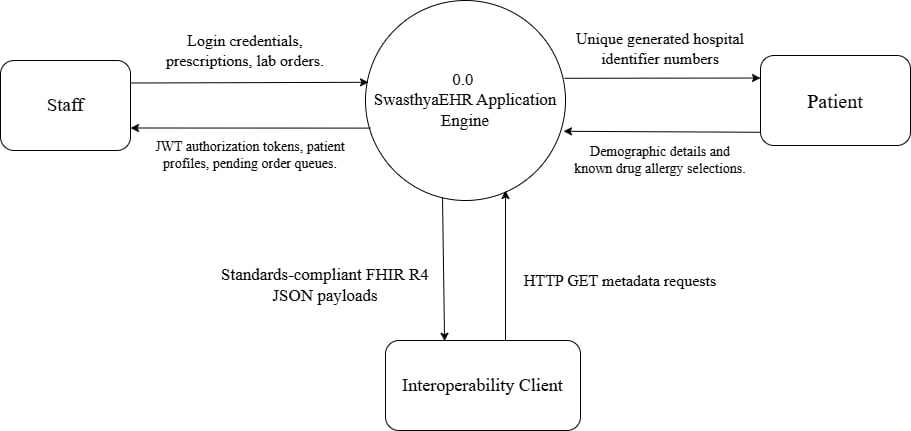
\includegraphics[width=1.05\textwidth]{Images/lvl0dfd.png}
\caption{Level 0 Data Flow Diagram of the System}
\label{fig:dfdlvl0}
\end{figure}

The Level 0 data flow diagram in Figure \ref{fig:dfdlvl0} gives the high-level view of the three external entities, which are the Staff, the Patient, and the Interoperability Client, sending requests to the system and receiving responses. The Staff entity feeds login credentials, prescriptions, and lab orders to the central system, which responds with JWT authorization tokens, patient profiles, and pending order queues. The Patient entity interacts by submitting demographic details and known drug allergy selections, receiving unique generated hospital identifier numbers in return. Finally, the Interoperability Client issues HTTP GET metadata requests to the SwasthyaEHR Application Engine, which streams back standards-compliant FHIR R4 JSON payloads to complete the data exchange.
\begin{figure}[H]
\centering
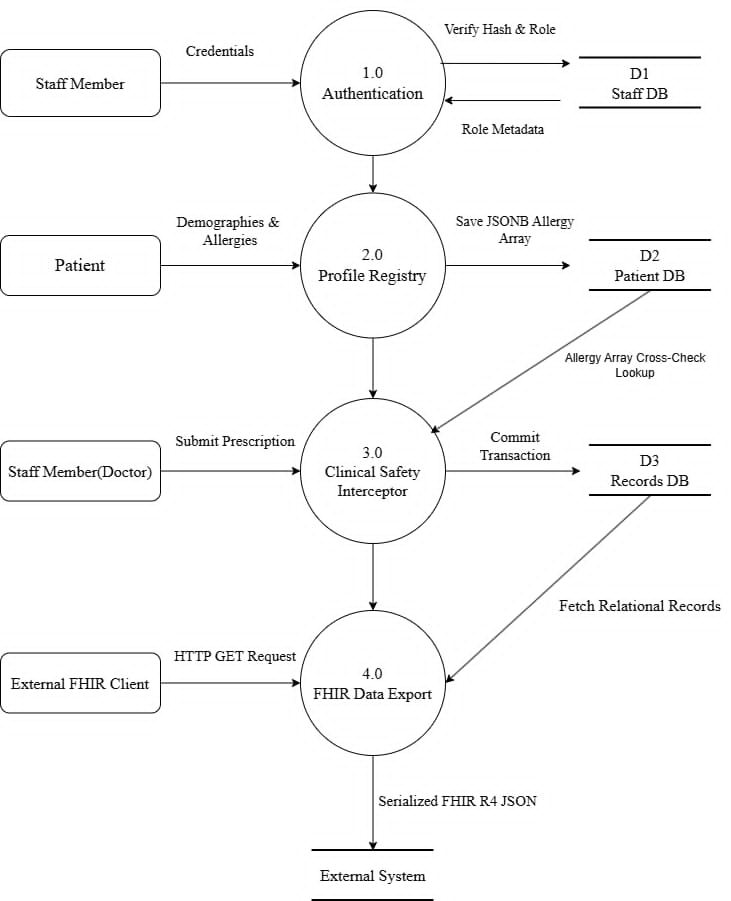
\includegraphics[width=1.0\textwidth]{Images/lvl1dfd.png}
\caption{Level 1 Data Flow Diagram of the System}
\label{fig:dfdlvl1}
\end{figure}

The system activity flowchart in Figure \ref{fig:flowchart} breaks the execution down into four main structural domains—the Doctor, the System/Backend Engine, the Pharmacist, and the Lab Technician—and shows how transactional data flows between them. When a doctor submits a prescription form, the Backend Engine routes the HTTP POST request through SimpleJWT middleware to validate the token signature and verify the user's role. If authorized, the engine opens an atomic database transaction and queries the PostgreSQL patient table to check the prescription name against the patient's recorded allergy substrings. If a match is found, the transaction is aborted and a red allergy warning banner is rendered on the frontend; otherwise, the system triggers a database commit to save the active prescription row, which instantly updates the doctor's dashboard and populates the pharmacy dispensing board for the pharmacist to fulfill. Concurrently, doctors can request lab tests, which streams electronic lab orders directly into the lab technician's work queue for numeric result submission, ensuring an audited, role-separated workflow from start to finish.
\subsection{System Flowchart}

\begin{figure}[H]
\centering
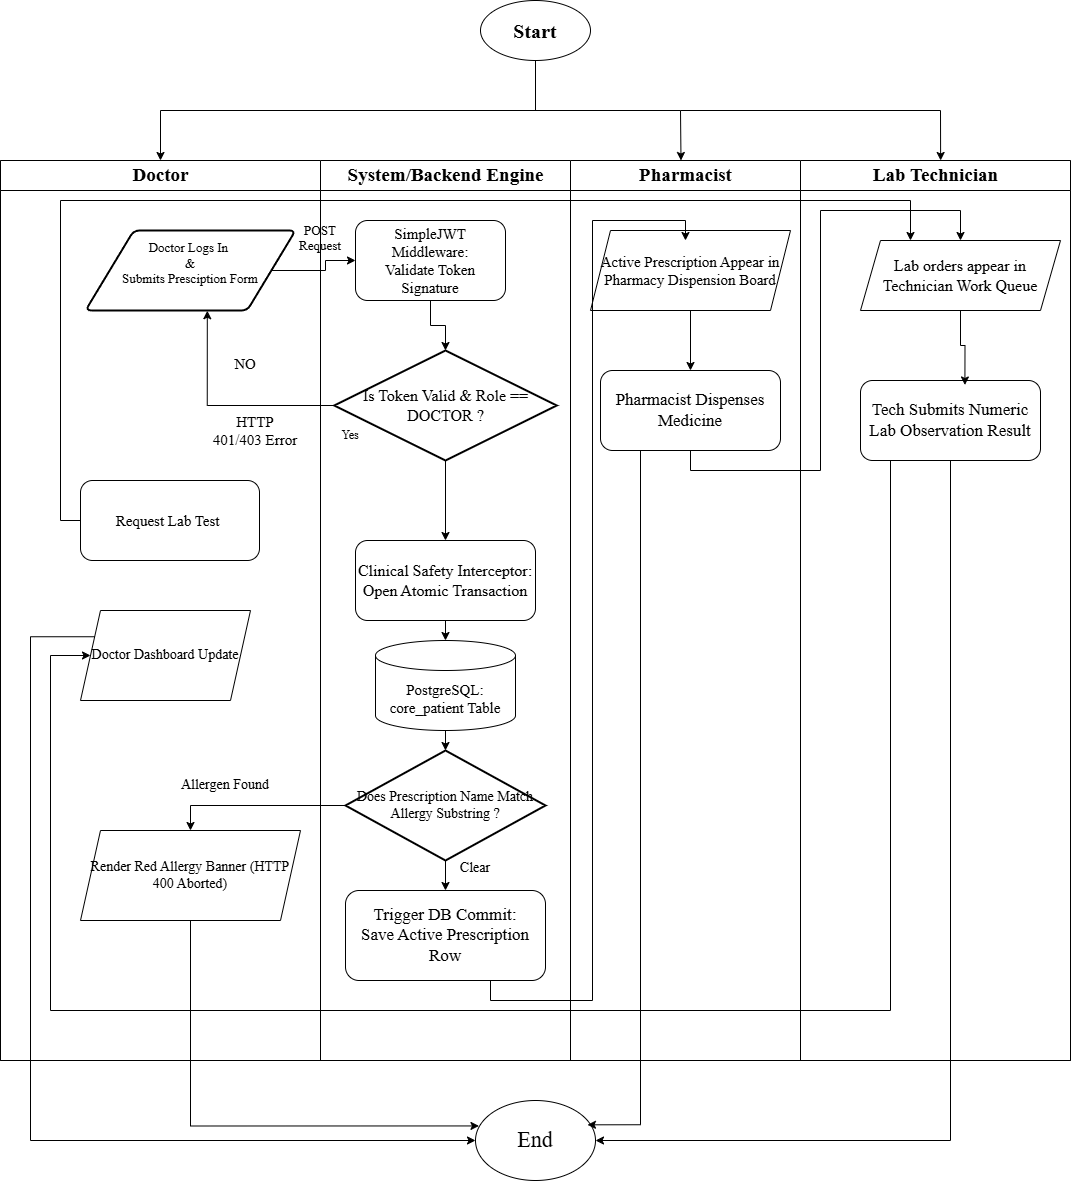
\includegraphics[width=1.14\textwidth]{Images/SystemFlowchart.png}
\caption{System Flowchart Showing Doctor, System/Backend Engine, and Pharmacist/Lab Technician Lanes}
\label{fig:flowchart}
\end{figure}

The activity flowchart in Figure \ref{fig:flowchart} shows the complete path that each user group follows from the moment they enter the system to the moment they leave. The flow starts at the top with a single start node and branches into four separate lanes representing different system roles and core processing layers: the Doctor, the System/Backend Engine, the Pharmacist, and the Lab Technician.

\textbf{Doctor Lane.} The doctor begins by entering credentials and submitting a prescription form. If the system returns an authentication error, the flow routes directly to the end node. If authorized, the doctor's interface remains on standby while the backend runs structural sweeps. If an allergen is found, the interface renders a red allergy banner alert before terminating. If the transaction is clear, the doctor's dashboard updates automatically. From this workspace, the doctor can also issue a laboratory test request, routing a digital order to auxiliary staff before logging out and reaching the end node.

\textbf{System/Backend Engine Lane.} This central processing lane manages validation rules and database transactional boundaries. When a prescription form is received via an HTTP POST request, the SimpleJWT middleware validates the token signature and verifies the doctor role. If invalid, it returns a 401/403 error and terminates. If valid, the clinical safety interceptor opens an isolated atomic transaction and queries the PostgreSQL patient table. The engine checks if the prescription name matches any stored allergy substrings. If a match occurs, it aborts the database transaction; if clear, it triggers a database commit to permanently save the active prescription row.

\textbf{Pharmacist and Lab Technician Lanes.} These auxiliary lanes manage specialized medical task queues driven by the backend database state. For the pharmacist, once a secure prescription row is committed by the backend engine, the active prescription immediately populates the pharmacy dispensing board, allowing the pharmacist to dispense the medication before the lane terminates at the end node. For the lab technician, when a doctor triggers a lab test request, the electronic order instantly appears in the technician's work queue. The technician then processes the patient sample, submits the numeric laboratory observation result back to the application engine, and finishes the cycle at the end node.

\section{Implementation Details}

\subsection{Frontend Development}

\begin{figure}[H]
\centering
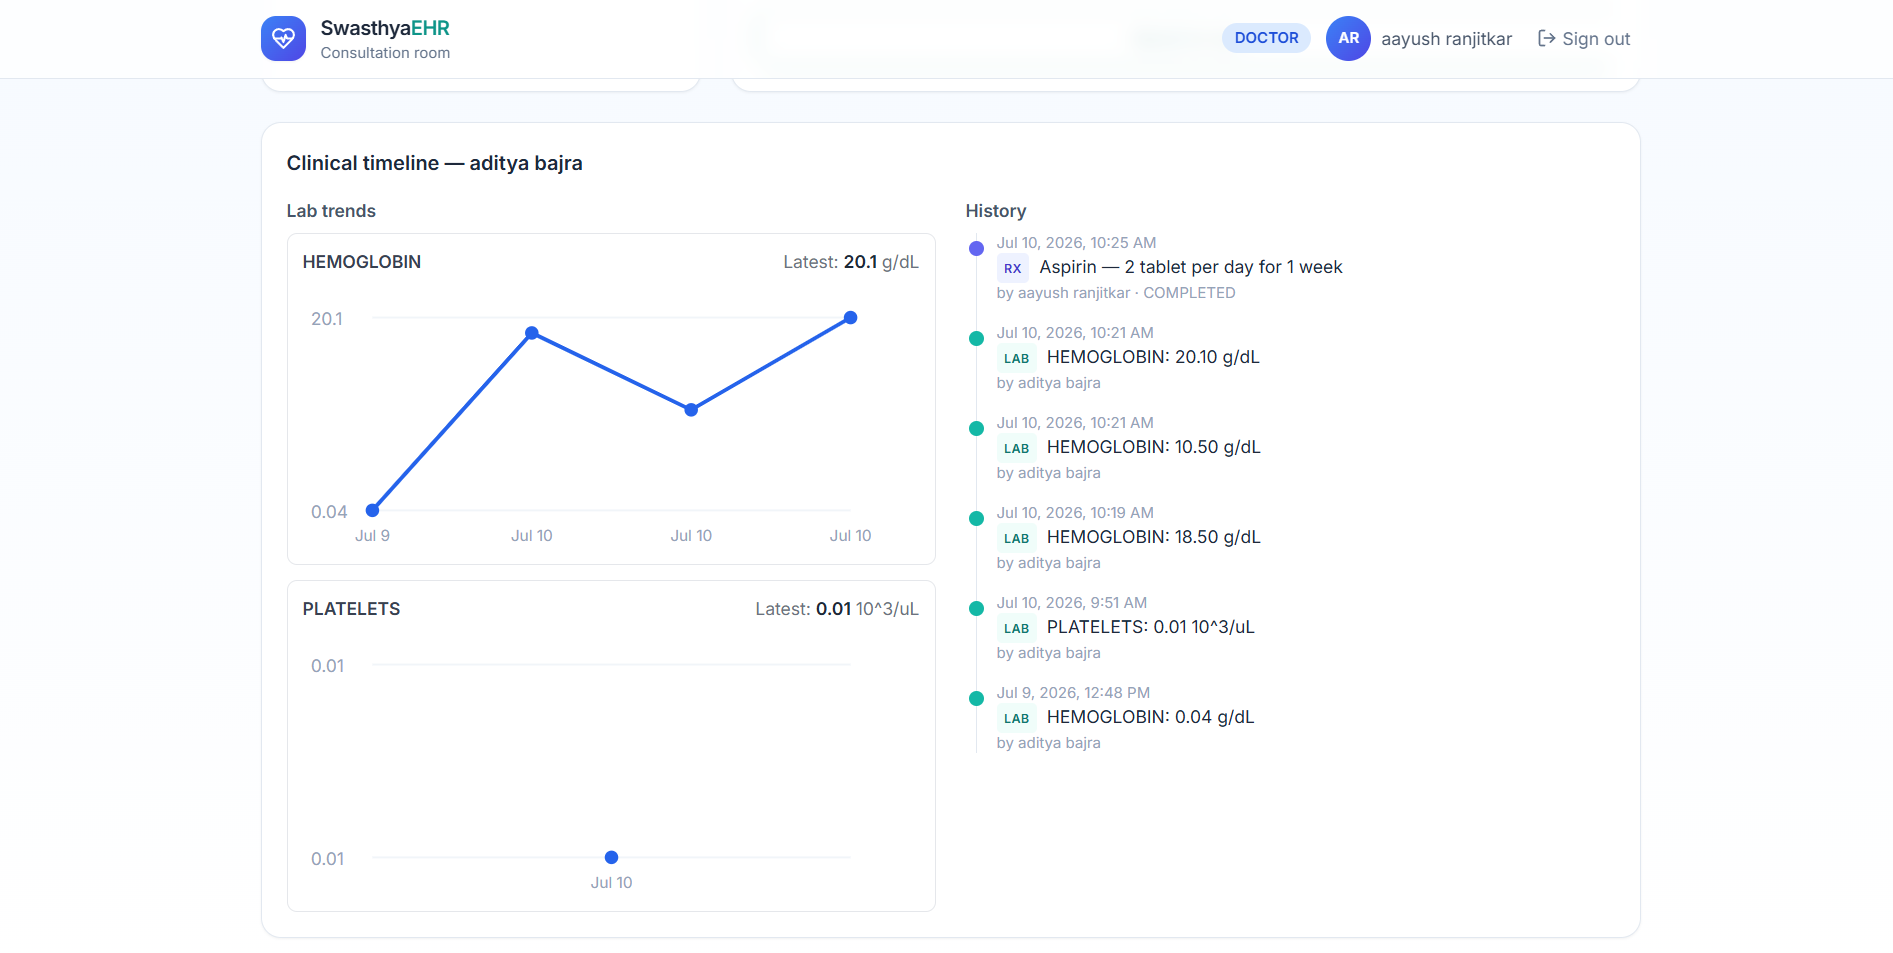
\includegraphics[width=0.9\textwidth]{Images/frontend.png}
\caption{Frontend of the Swasthya-EHR Platform}
\label{fig:Frontend}
\end{figure}
The frontend is a React-based single-page application that talks to the backend through JSON HTTP requests. It is built for four types of users, which are patient, doctor, technician, and pharmacist, along with a secure administrative dashboard that handles user management. The patient side handles registration, six-digit email verification code processing, login, and longitudinal health summaries that display trends of vital markers aggregated over time. The doctor side features a clinical registry dashboard where the user can query active patient nodes, review historical laboratory timelines, and issue new medication prescriptions. The technician side provides targeted forms to input raw numerical laboratory findings and automatically attach standard system markers. The pharmacist side provides a verification console to view active prescriptions and log fulfillment status. The administrative panel features controls to manage database accounts, modify user profiles, and assign Role-Based Access Control (RBAC) levels. The interface layout leverages Tailwind CSS utility classes to guarantee that viewports adapt seamlessly across hospital terminals, tablet units, and mobile devices, while toast components provide real-time notification alerts for validation updates.

\subsection{Backend Development}
The backend is built with Python and the Django REST Framework (DRF), which together handle HTTP requests, routing, business logic, and authentication filters. The database is PostgreSQL, and it is accessed through Django's native Object-Relational Mapping (ORM) engine, which keeps the schema clean and handles database migrations automatically. For login, the system utilizes JSON Web Tokens (JWT) where the Django engine generates a cryptographically signed token incorporating user identification claims and explicit role assignments. The application routes are tightly split based on user authorization boundaries. Patient routes handle account creation, email verification code tracking, password updates, and longitudinal metric streaming. Provider routes manage patient indexing, prescription generation, and laboratory result uploads, while admin routes are strictly guarded to restrict user manipulation privileges to verified administrators. Custom middleware protects endpoints that require a logged-in session, Django serializers validate the data structure schema inputs, and a centralized exception handler maps errors into clean JSON responses. The codebase is structurally organized into distinct, modular layers for models, views, serializers, middleware, and interoperability tools.

\subsection{Interoperability and Clinical Validation Integration}
The interoperability and safety validation layer is built into the Django backend using custom parsing scripts and transaction managers. The data transformation pipeline dynamically maps incoming flat relational rows into valid HL7 FHIR R4 JSON resources, converting local laboratory testing keywords into globally accepted LOINC and SNOMED CT terminology codes. When a technician submits a new test result, the parsing layer embeds the variables into standardized Patient and Observation resource payloads on the fly. Clinical safety boundaries are enforced directly within the application code by wrapping prescription operations inside isolated database transactions using the \texttt{@transaction.atomic} decorator. When a doctor writes a new medication order, the backend interceptor catches the text input, changes the casing to lowercase, and compares the drug string against the patient's recorded allergy array using case-insensitive substring matching. If a text intersection is found, the validation engine throws a severe error, and Django automatically triggers a database rollback to erase the uncommitted write block and protect the data from entering a corrupted state.

\subsection{Database Schema}
The database is PostgreSQL and it is managed through Django's built-in migration utility, with all architectural variations version-controlled in standard tracking files. Currently, the schema contains two primary relational tables, which are users, which holds name, email, password hash, role classification, and verified flags, and verification\_codes, which stores the six-digit validation code, expiration timestamp, and a foreign key mapping back to the user with cascade delete constraints. The patient profile table incorporates standard structured attributes for demographics alongside a specialized JSONB binary data column designed to store the variable-length array of text allergens. The schema will be systematically extended in the final phase to include dedicated, indexed relational tables for longitudinal FHIR observations, historical doctor prescriptions, lab technician entries, and system-wide security audit logs.

\subsection{Testing Strategy}
\begin{itemize}
    \item \textbf{Unit Testing:} Each independent code module is verified on its own. This covers password hashing algorithms, verification code generation, input serialization schemas, Django ORM table lookups, React interface state changes, and the FHIR mapping functions using mock clinical datasets.
    \item \textbf{Integration Testing:} Component interactions are verified together as a single flow, such as user registration generating an account entry and an active verification code simultaneously, JWT handling route access states, the RBAC middleware blocking unauthorized profile modifications, and the data pipeline bridging the backend, database, and frontend.
    \item \textbf{User Acceptance Testing:} Real testing groups interact with the application screens and provide operational feedback. Medical personnel test patient lookup and prescription writing workflows, while simulated patients test registration and longitudinal trend views.
    \item \textbf{Performance Testing:} API response thresholds for data mapping and security intercepts are measured to keep execution latency under two seconds, the system is validated under high concurrent transaction loads, and rendering alignment is checked across multiple web browsers and screen dimensions.
\end{itemize}
%----------------------------------------------------------------------
% CHAPTER 4: EXPECTED OUTPUT
%----------------------------------------------------------------------
\chapter{Results and Discussion}

This chapter is divided into two parts. The first part lists the work that has been com-
pleted by the mid term defense and is already visible in the current code repository. The
second part lists the work that is still in progress and is planned for the next project
phase.

\section{Task Completed}

This section details the fully implemented and operational architectural components of the SwasthyaEHR ecosystem. The development was executed across a decoupled, client-server architecture bound by strict types and semantic clinical schemas.

\subsection{Backend System Architecture (Django 5, DRF, and PostgreSQL)}
The backend engineering layer utilizes Python 3 with Django 5 and Django REST Framework (DRF), backed by a production-ready PostgreSQL instance managed through Django’s native Object-Relational Mapping (ORM). The finalized server infrastructure comprises the following structural components:
\begin{itemize}
    \item \textbf{Custom User Model and Cryptographic Auth Architecture:} A unified \texttt{Staff} identity schema replaces the default user model, integrating an explicit role attribute. Authentication is driven via secure cryptographic token assertions using standard JSON Web Tokens (JWT). The system handles user registration, session management, secure password hashing, and token issuance where user scopes are encapsulated directly inside the token payload.
    \item \textbf{Granular Role-Based Access Control (RBAC):} Enforcement of operational scopes is achieved via a reusable server-side \texttt{EnforceStrictRole} permission filter class. Every REST endpoint declares its allowed role array explicitly; this authorization middleware intercepts incoming queries at the server boundary, preventing any client-side UI bypass.
    \item \textbf{Optimized Patient Registry and Indexing:} Patient profiles use universally unique identifiers (UUIDs) as primary keys and feature an auto-generated, sequential institution identifier format (\texttt{HOSP-YYYY-NNNNN}). A \texttt{registered\_by} tracking field enables a dual-channel intake pipeline, supporting both public client self-registration and receptionist-driven administrative intake. Patient allergy rosters are serialized directly as a PostgreSQL \texttt{JSONB} document field, equipped with a \texttt{GIN} (Generalized Inverted Index) to guarantee sub-millisecond keyword lookup speeds.
    \item \textbf{Standardized Laboratory and Clinical Observation Subsystem:} An active diagnostic tracking engine handles \texttt{LabOrder} (physician intent) and \texttt{LabObservation} (technician results) entities. The data pipeline maps relational database rows on the fly to universal semantic vocabularies. It actively parses three specific core laboratory parameters, binding them tightly to official Logical Observation Identifiers Names and Codes (LOINC):
    \begin{itemize}
        \item \textit{Hemoglobin} (LOINC: \texttt{718-7}), bound to precise reference ranges and SI units.
        \item \textit{White Blood Cell Count (WBC)} (LOINC: \texttt{6690-2}), with integrated validation boundaries.
        \item \textit{Platelets} (LOINC: \texttt{777-3}), equipped with mathematical threshold triggers.
    \end{itemize}
    \item \textbf{Atomic Clinical Safety Interceptor and Prescription Engine:} The prescription module features an active safety wrapper executed under an explicit isolation boundary using Django's \texttt{@transaction.atomic} decorator. When a physician submits a prescription, the interceptor executes a real-time substring matching sweep between the incoming drug string and the patient's indexed allergy array. If a collision is detected, the database write is instantly aborted, rolling back the transaction and dispatching a structured HTTP 400 bad-request alert payload. Safe transactions persist in an \texttt{ACTIVE} status, exposing them to an institutional fulfillment pipeline that transitions them to \texttt{COMPLETED} upon pharmacist dispensing.
    \item \textbf{HL7 FHIR R4 Interoperability Serialization Engine:} The system features read-only endpoints dedicated to healthcare semantic translation. These components map internal relational models directly into compliant, standardized JSON profiles, serving payloads under the official \texttt{application/fhir+json} content-type header. Implemented resources include the structural \texttt{Patient} registry schema, standalone clinical \texttt{Observation} blocks, and a combined \texttt{Patient/\$everything} structural transaction \texttt{Bundle}.
    \item \textbf{Aggregated Clinical Timeline Engine:} A specialized timeline extraction utility merges disjointed transactional tables (prescriptions, laboratory tests, and vitals) chronologically. This engine powers cross-institutional health profile collation and parses historical data points to expose longitudinal lab-value trend trajectories.
\end{itemize}

\subsection{Frontend Architecture and Interface Design (React 18, Vite, and Tailwind CSS)}
The user interface is engineered as a highly responsive single-page application (SPA) using React 18 and Vite, structured visually through Tailwind CSS utility classes. The client architecture transitions hardcoded diagnostic views into reactive components through the following features:
\begin{itemize}
    \item \textbf{Role-Tailored Operational Spaces:} The frontend maps to the system's backend security scopes by deploying six distinct, role-themed workspaces. Each interface is distinctively color-coded to reduce operational errors during high-throughput workflows:
    \begin{itemize}
        \item \textbf{Administrative Control Panel:} Dedicated to system monitoring, logging, and granular staff identity management.
        \item \textbf{Receptionist Portal:} Optimized for fast patient intake, self-registration verification, and profile indexing.
        \item \textbf{Physician Dashboard:} Equipped with unified patient lookups, active electronic prescribing widgets, lab order dispatch controls, and visual trend line charts charting clinical histories over time.
        \item \textbf{Laboratory Interface:} A specialized diagnostic queue enabling technicians to pull pending orders and submit numeric data via range-hinted, validation-locked input forms.
        \item \textbf{Pharmacy Dispensing Board:} A live, reactive fulfillment grid displaying active medical prescriptions ready for verification and handoff.
        \item \textbf{Patient Portal:} A secure, read-only dashboard allowing individuals to review their aggregated timeline and export their medical bundle records.
    \end{itemize}
    \item \textbf{Enhanced Authentication UI Controls:} A modern split-screen sign-in interface includes an absolute toggle separating Patient and Staff entryways. The registration interface utilizes a multi-step design pattern complete with strict client-side validations to filter formatting errors before data hit the network.
    \item \textbf{Reusable Component System:} To maximize interface cohesion and optimize user experience, several high-utility components were introduced:
    \begin{itemize}
        \item \textbf{Verification Input Node:} Features automated focus-forward shifting, paste event interception, backspace-driven backward navigation, and an inline resend countdown timer.
        \item \textbf{Global Toast Notification Stack:} A modular notification center that intercepts backend API responses to stream standardized, real-time success banners or error feedback alerts inline.
        \item \textbf{Static Card and Analytical Matrices:} Preconfigured visualization structures populated with dynamic telemetry counters and data-driven line charts ready for seamless integration with real-time API endpoints.
    \end{itemize}
\end{itemize}


\section{Task remaining}

\subsection{Expanded Laboratory Diagnostics and LOINC Mapping}
The initial implementation of the laboratory subsystem supports a three-test baseline (Hemoglobin, White Blood Cell Count, and Platelets) as a functional proof of concept for a Complete Blood Count (CBC). To transition this module into a comprehensive diagnostic suite, the data architecture is being extended by expanding the system's Logical Observation Identifiers Names and Codes (LOINC) reference table. 

Because the underlying verification engine, relational storage layers, and FHIR serialization pipelines were built to be data-agnostic, onboarding new diagnostic panels requires only defining their respective LOINC codes, measurable units, and reference ranges. The planned expansion panels are detailed in Table~\ref{tab:loinc_expansion}.

\begin{table}[htbp]
\centering
\caption{Planned Laboratory Panel Extensions with LOINC Standardization}
\label{tab:loinc_expansion}

\begin{tabularx}{\textwidth}{|l|X|l|}
\hline
\textbf{Diagnostic Panel} & \textbf{Target Measurands / Observations} & \textbf{Target LOINC Reference} \\ \hline
Complete Blood Count (Full) & RBC, Hematocrit, MCV, MCH, MCHC & 789-8, 4544-3, 787-2 \\ \hline
Blood Glucose Matrix & Fasting Blood Sugar, Random Blood Sugar & 1558-6, 2339-0 \\ \hline
Glycated Haemoglobin (HbA1c) & Total HbA1c (Diabetes Monitoring Baseline) & 4548-4 \\ \hline
Lipid Profile Suite & Total Cholesterol, LDL, HDL, Triglycerides & 2093-3, 2089-1, 2085-9 \\ \hline
Kidney Function Test (KFT) & Serum Creatinine, Blood Urea Nitrogen, Urea & 2160-0, 3091-6, 3094-0 \\ \hline
Liver Function Test (LFT) & ALT, AST, Total Bilirubin & 1742-6, 1920-8, 1975-2 \\ \hline
Thyroid Profile & TSH, Free T3, Free T4 & 3016-3, 3053-6, 3024-7 \\ \hline
Serum Electrolytes & Sodium, Potassium, Chloride & 2951-2, 2823-3, 2075-0 \\ \hline
\end{tabularx}

\end{table}
\clearpage
\subsection{Expanded FHIR Interoperability Layer}
While the current export engine successfully serializes \texttt{Patient} registries, independent \texttt{Observation} resources, and localized transaction \texttt{Bundle} models, a more comprehensive data graph is required for deep ecosystem integration. Current development focus is directed toward implementing the following interoperability layers:
\begin{itemize}
    \item \textbf{MedicationRequest Integration:} Automatically serializing active electronic prescriptions generated by the physician interface into fully structured FHIR resources.
    \item \textbf{ServiceRequest Pipelines:} Encoding electronic laboratory orders to track diagnostic intents cleanly from initial request through technician fulfillment.
    \item \textbf{DiagnosticReport Aggregation:} Structuring an wrapper resource to group multiple underlying numeric clinical observations into single, unified laboratory reports.
    \item \textbf{Practitioner Profiles:} Attaching authenticated clinician and staff metadata to records to satisfy institutional provenance and auditing demands.
    \item \textbf{One-Click Local Extraction:} Provisioning a user interface control that enables users to download their complete health record profile instantly as a standardized, encrypted JSON bundle.
\end{itemize}
To validate this interoperability framework, the serialized payloads will be systematically tested against the official HL7 FHIR Validator and Inferno test suites to ensure strict compliance with global specifications.

\subsection{Symptom-Based Registration and Deterministic Routing}
To bridge the gap between patient intake and specialized clinical workflows, a deterministic routing module is being integrated into the registration sequence. This enhancement optimizes patient flows while strictly avoiding automated clinical diagnostics:
\begin{itemize}
    \item \textbf{Chief Complaint Ingestion:} During profile intake, patients provide a free-text narrative of their primary symptom (e.g., ``persistent cough'', ``acute chest pain'') and select an operational department from an explicit dropdown menu.
    \item \textbf{Rule-Based Direction Mapping:} A simple, transparent routing matrix maps generalized complaint classes directly to medical specialties (e.g., mapping chest pain directly to Cardiology, or localized rashes to Dermatology) for triage efficiency.
    \item \textbf{Queue Population:} Following specialty assignment, the patient selects from an active directory of available clinicians, generating a lightweight \texttt{Appointment/Visit} entity that populates the selected physician's real-time dashboard queue without persisting disease or diagnostic codes.
\end{itemize}

\subsection{Deterministic Risk Analysis and Clinical Safety Flags}
Rather than deploying black-box machine learning models to infer clinical conditions, this project introduces a rule-based, fully explainable risk-flagging subsystem. By cross-referencing structured data entries—such as lab trends, patient age bounds, and concurrent active ingredients—the system surfaces critical insights directly to the care provider:
\begin{itemize}
    \item \textbf{Dynamic Laboratory Boundary Flags:} Comparing telemetry directly against LOINC reference ranges to display real-time, color-coded warning badges (\textit{Low, Normal, High, Critical}) within the patient chart layout.
    \item \textbf{Critical-Value Safety Triggers:} Isolating dangerous biometric drops to trigger structural flags (e.g., mapping an extreme drop in Platelets to a critical ``Bleeding-Risk Alert'' banner) to maximize proactive response times.
    \item \textbf{Comprehensive Profile Risk Overlays:} Scaling the existing atomic safety interceptor to provide highly visible, cross-institutional allergy warning summaries across the main workspace profile.
    \item \textbf{Polypharmacy Alerts:} Evaluating active medication rosters to alert physicians when a patient crosses a threshold of concurrent active prescriptions, mitigating adverse drug-drug interactions.
    \item \textbf{Demographic Variance Safety Bands:} Parsing demographic dates of birth to apply explicit care-banding flags for pediatric or geriatric cohorts, prompting specialized dosing consideration.
    \item \textbf{Lab-Trend Trajectory Monitoring:} Evaluating chronologically sequenced lab rows over an integrated timeline to visually flag when a tracked physiological marker is deteriorating across successive institutional visits.
\end{itemize}

%----------------------------------------------------------------------
% REFERENCES
%----------------------------------------------------------------------
\renewcommand{\bibname}{References}
\begin{thebibliography}{99}
\addcontentsline{toc}{chapter}{References}

\bibitem{bates1}
D. W. Bates, M. Cohen, L. L. Leape, J. M. Overhage, M. M. Shabot, and T. Sheridan. Reducing the Frequency of Errors in Medicine Using Information Technology. \textit{Journal of the American Medical Informatics Association}, 8(4):299--308, 2001. doi: 10.1136/jamia.2001.0080299.

\bibitem{bates2}
D. W. Bates, L. L. Leape, D. J. Cullen, E. Laird, L. A. Petersen, S. D. Teich, E. Burdick, M. Hickey, S. Kleefield, B. Shea, M. Vander Vliet, and D. L. Seger. Effect of Computerized Physician Order Entry and a Team Intervention on Prevention of Serious Medication Errors. \textit{JAMA}, 280(15):1311--1316, 1998. doi: 10.1001/jama.280.15.1311.

\bibitem{adler}
J. Adler-Milstein, A. J. Holmgren, P. Kralovec, C. Worzala, T. Searcy, and V. Patel. Electronic Health Record Adoption in US Hospitals: The Emergence of a Digital "Advanced Use" Divide. \textit{Journal of the American Medical Informatics Association}, 24(6):1142--1148, 2017. doi: 10.1093/jamia/ocx080.

\bibitem{bender}
D. Bender and K. Sartipi. HL7 FHIR: An Agile and RESTful Approach to Healthcare Information Exchange. In \textit{Proceedings of the 26th IEEE International Symposium on Computer-Based Medical Systems (CBMS)}, pp. 326--331, 2013. doi: 10.1109/CBMS.2013.6627810.

\bibitem{mandel}
J. C. Mandel, D. A. Kreda, K. D. Mandl, I. S. Kohane, and R. B. Ramoni. SMART on FHIR: A Standards-Based, Interoperable Apps Platform for Electronic Health Records. \textit{Journal of the American Medical Informatics Association}, 23(5):899--908, 2016. doi: 10.1093/jamia/ocv189.

\bibitem{hl7spec}
HL7 International. HL7 FHIR Release 4 (R4) Specification. Available: \url{https://hl7.org/fhir/R4/}. Accessed: 2026-03-10.

\bibitem{loinc}
C. J. McDonald, S. M. Huff, J. G. Suico, G. Hill, D. Leavelle, R. Aller, A. Forrey, K. Mercer, B. DeMoor, T. Hook, et al. LOINC, A Universal Standard for Identifying Laboratory Observations: A 5-Year Update. \textit{Clinical Chemistry}, 49(4):624--633, 2003. doi: 10.1373/49.4.624.

\bibitem{kuperman}
G. J. Kuperman, A. Bobb, T. H. Payne, A. J. Avery, T. K. Gandhi, G. Burns, D. W. Bates, and D. K. Kaushal. Medication-Related Clinical Decision Support in Computerized Provider Order Entry Systems: A Review. \textit{Journal of the American Medical Informatics Association}, 14(1):29--40, 2007. doi: 10.1197/jamia.M2170.

\bibitem{vandersijs}
H. van der Sijs, J. Aarts, A. Vulto, and M. Berg. Overriding of Drug Safety Alerts in Computerized Physician Order Entry. \textit{Journal of the American Medical Informatics Association}, 13(2):138--147, 2006. doi: 10.1197/jamia.M1809.

\bibitem{topaz}
M. Topaz, D. L. Seger, S. P. Slight, A. Goss, T. Lai, and D. W. Bates. Rising Drug Allergy Alert Overrides in Electronic Health Records: An Observational Retrospective Study of a Decade of Experience. \textit{Journal of the American Medical Informatics Association}, 23(3):601--608, 2016. doi: 10.1093/jamia/ocv114.

\bibitem{possible}
Possible Health. Open-Source Electronic Health Record Deployment at Bayalpata Hospital, Nepal. Available: \url{https://possiblehealth.org/}. Accessed: 2026-03-15.

\bibitem{dhis2}
HISP Centre, University of Oslo. DHIS2: District Health Information Software 2. Available: \url{https://dhis2.org/}. Accessed: 2026-03-15.

\bibitem{who}
World Health Organization. \textit{Global Strategy on Digital Health 2020--2025}. Geneva: World Health Organization, 2021.

\bibitem{mohp}
Ministry of Health and Population, Government of Nepal. \textit{Nepal Health Sector Strategy 2015--2020}. Kathmandu, Nepal, 2015.

\end{thebibliography}

\chapter{Appendix}

\begin{figure}[H]
\centering
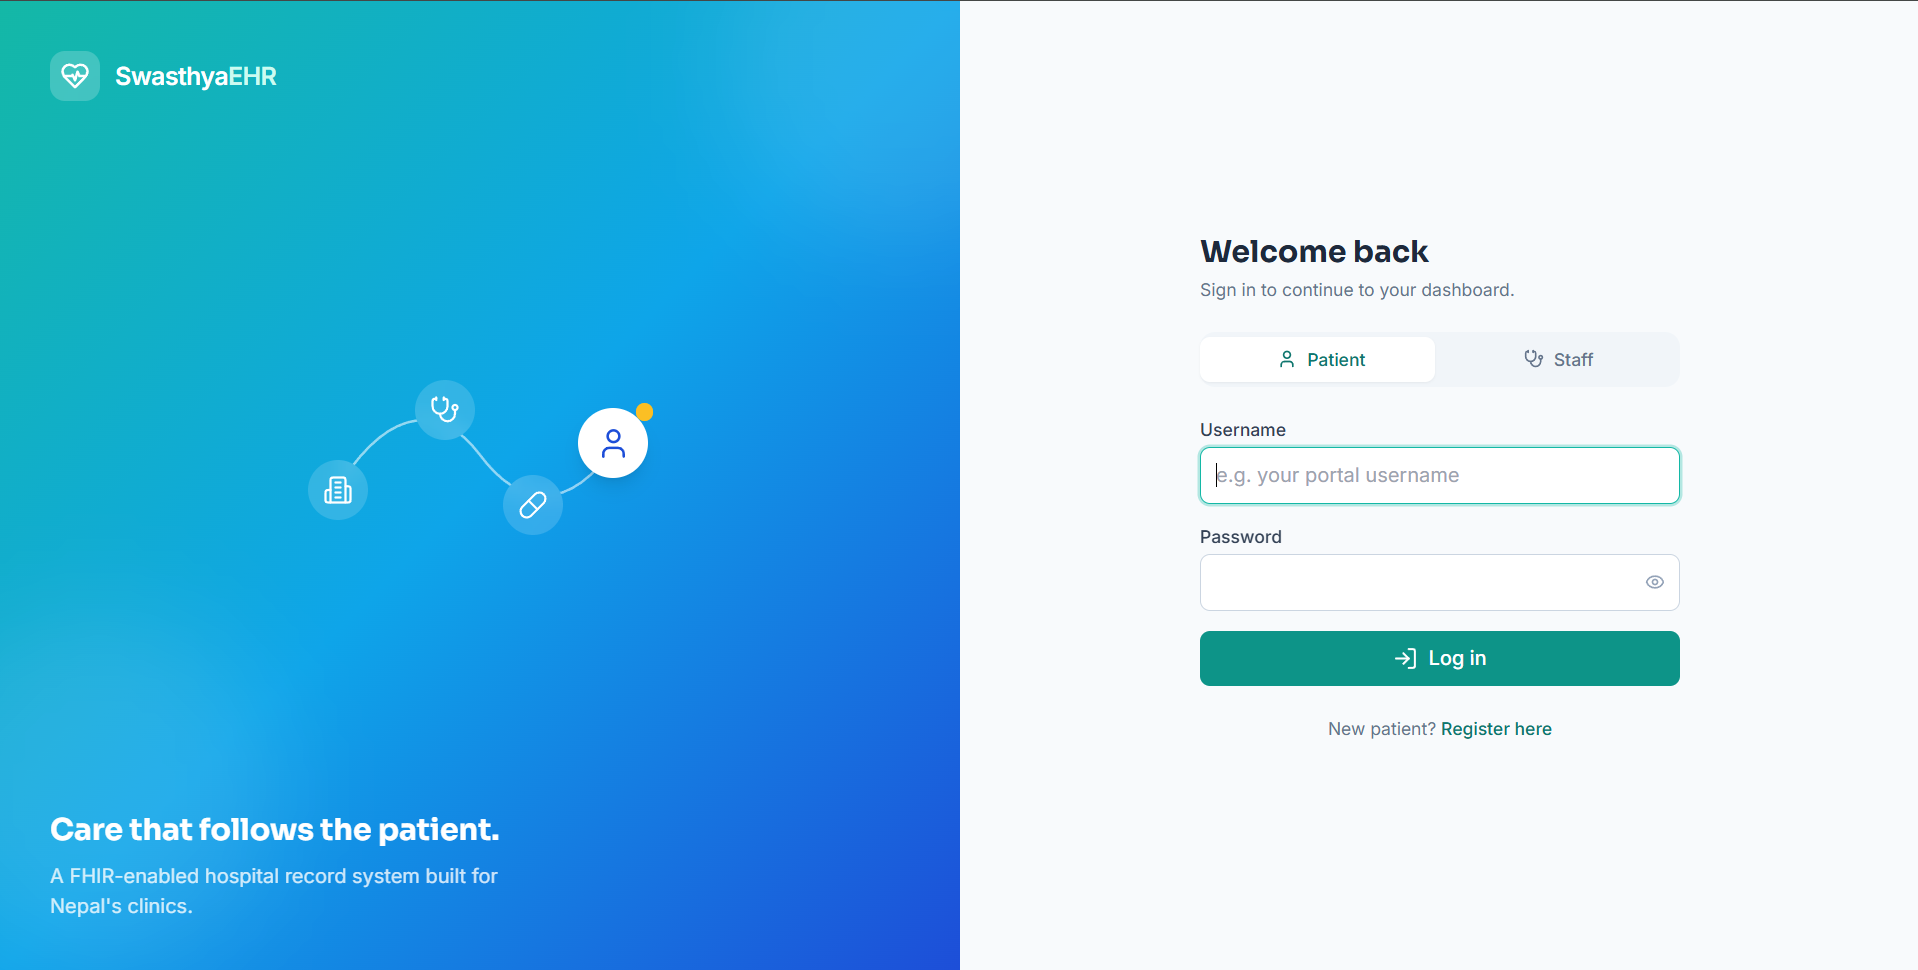
\includegraphics[width=1.0\textwidth]{Images/f1.png}
\caption{Login page}
\label{fig:Login}
\end{figure}

\begin{figure}[H]
\centering
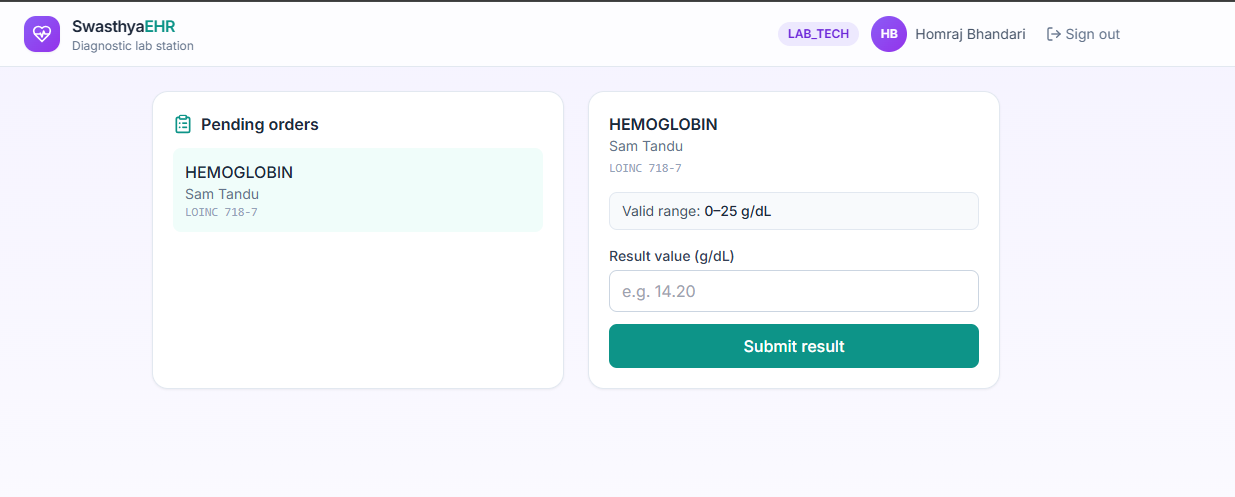
\includegraphics[width=1.0\textwidth]{Images/labd.png}
\caption{Lab Technician Dashboard}
\label{fig:LabTechnician}
\end{figure}

\begin{figure}[H]
\centering
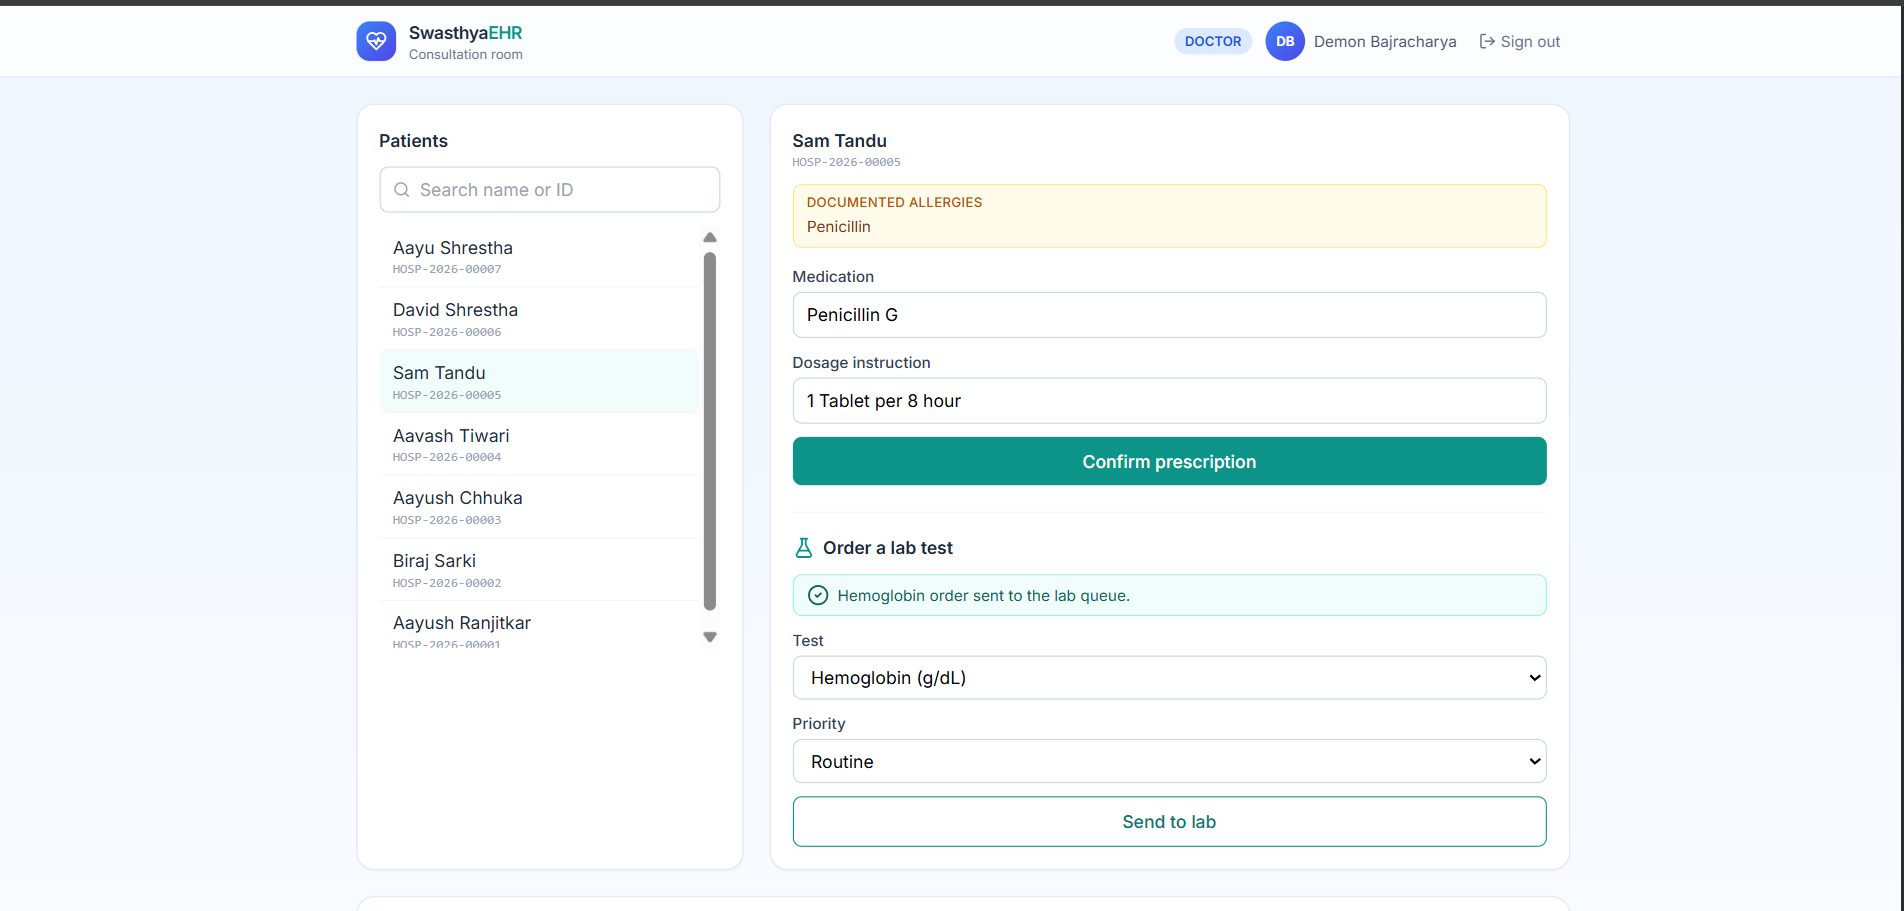
\includegraphics[width=1.0\textwidth]{Images/doctord.png}
\caption{Doctor Dashboard}
\label{fig:Doctor}
\end{figure}

\begin{figure}[H]
\centering
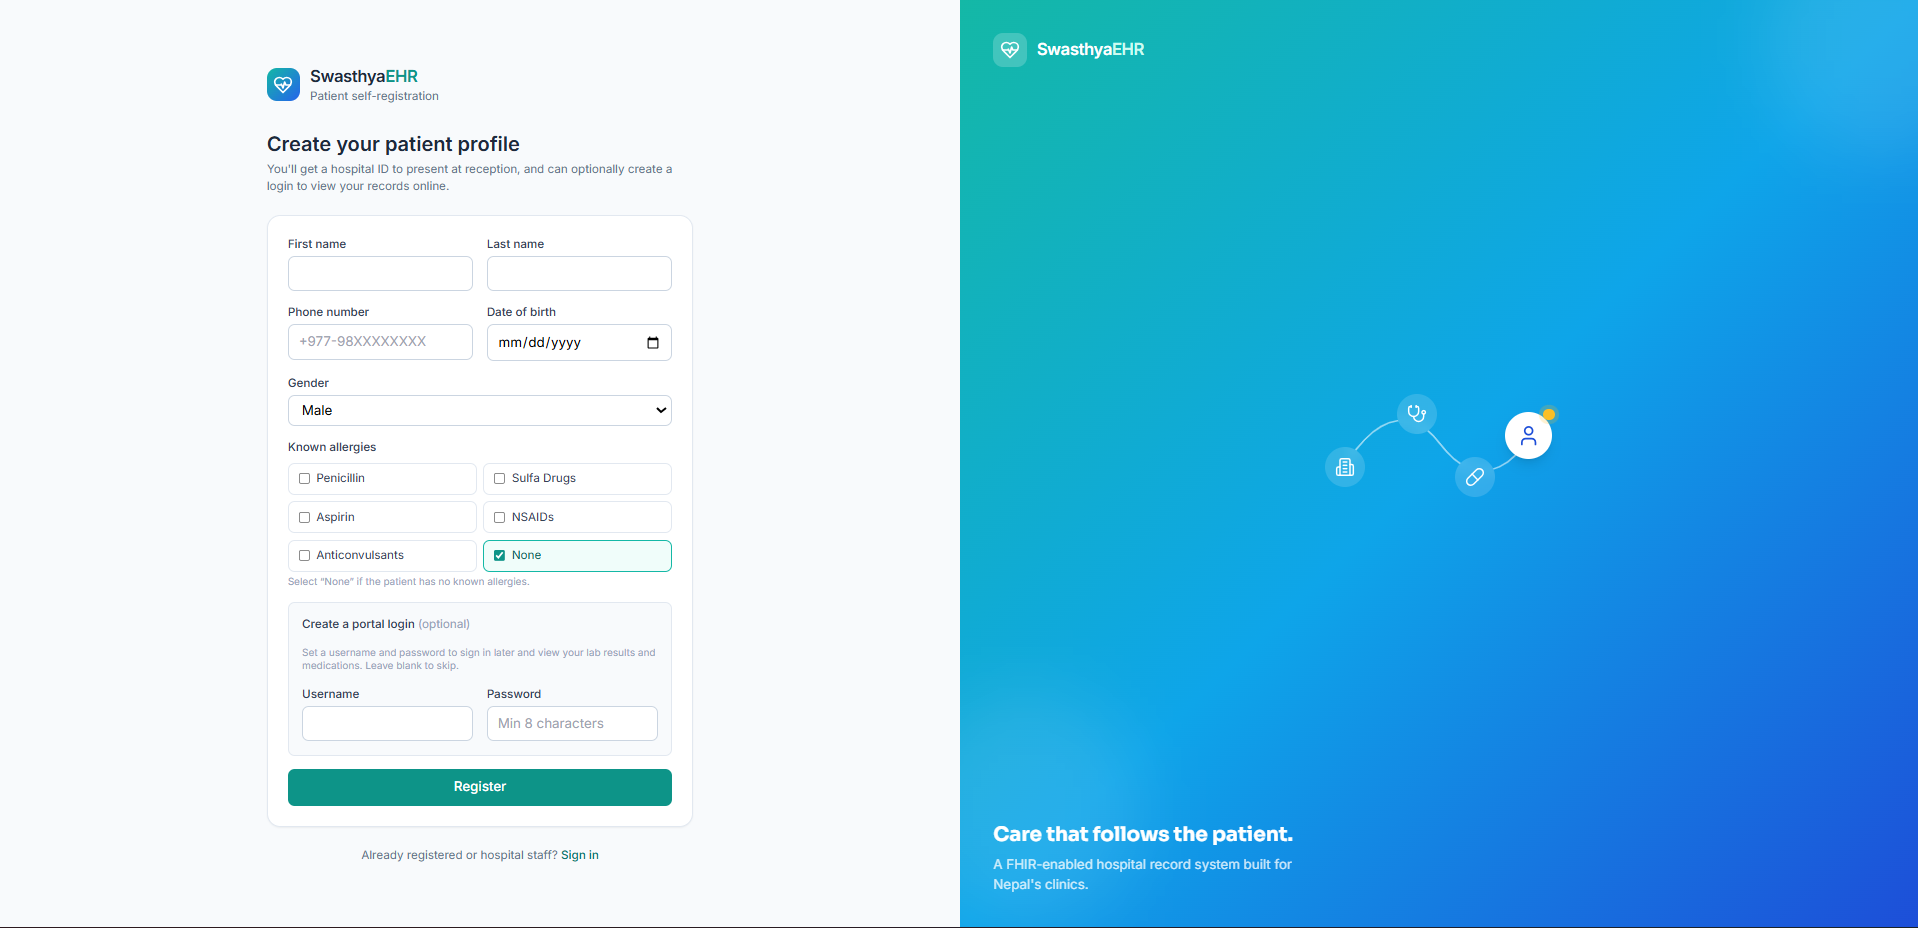
\includegraphics[width=1.0\textwidth]{Images/reg.png}
\caption{PatientRegistration Page}
\label{fig:Registration}
\end{figure}

\begin{figure}[H]
\centering
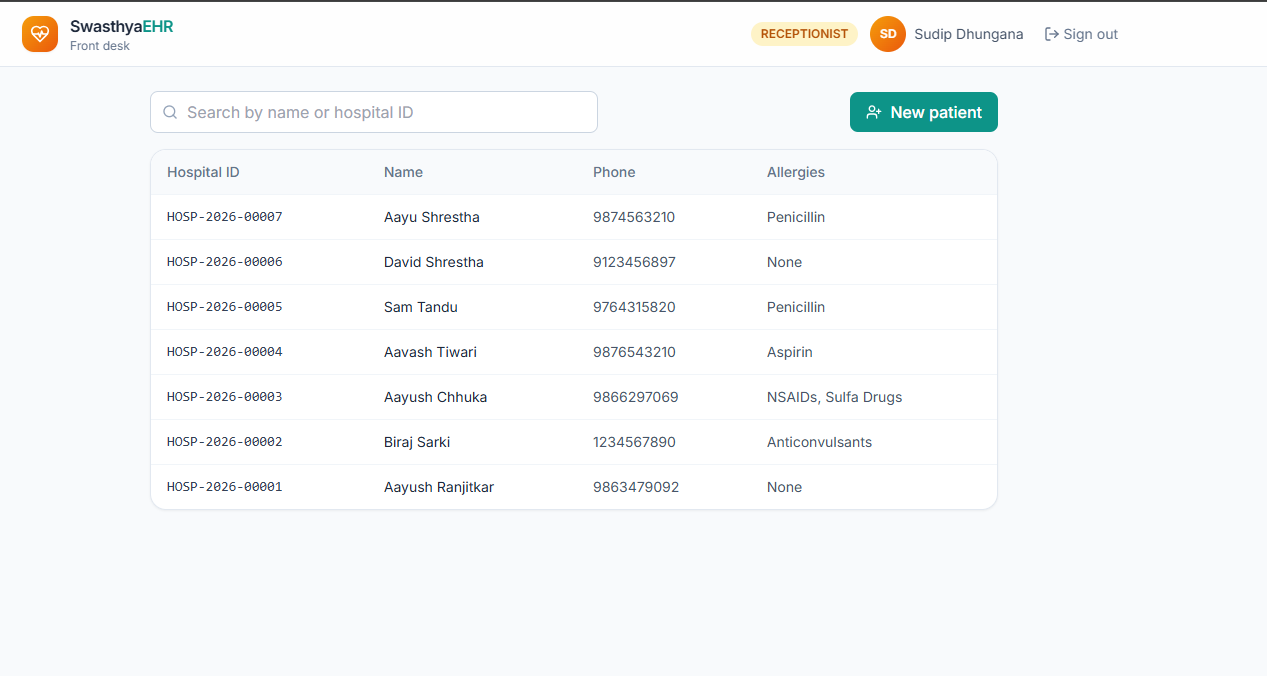
\includegraphics[width=1.0\textwidth]{Images/recep.png}
\caption{Receptionist Dashboard}
\label{fig:Registration}
\end{figure}
                                                                          

\end{document}
